\chapter{听觉处理的中枢神经系统}
听觉对于定位和识别声音至关重要; 对于人类来说,它特别重要,因为它在理解和产生语言方面发挥着重要作用。 听觉系统有几个值得注意的特征。 它的皮层下通路比其他感觉系统的通路更长。 与视觉系统不同,声音可以从四面八方进入听觉系统,白天和黑夜,无论我们睡着还是醒着。 听觉系统不仅处理从体外发出的声音(环境声音、他人发出的声音),还处理自己产生的声音(发声和咀嚼声音)。 声音刺激在空间中的位置不是由感觉传入神经元的空间排列来传达的,而是由听觉系统根据物理线索的表示来计算的。

\section{声音向有听觉的动物传达多种类型的信息}
听觉有助于提醒动物注意看不见的危险或机会的存在,而且在许多物种中,听觉还可以作为一种交流方式。 必须从每只耳朵的声音物理特性表示中提取有关声音从何处产生及其含义的信息。 要了解动物如何处理声音,首先要考虑哪些线索可用。

大多数脊椎动物利用两只耳朵来定位水平面上的声音。 在该平面上不同位置的声源对两只耳朵的影响不同:声音到达较早,并且在靠近声源的耳朵处更强烈(图\ref{fig:localizing})。 双耳时间和强度差异携带有关声音出现位置的信息。

% !htb
\begin{figure}[htbp]
	\centering
	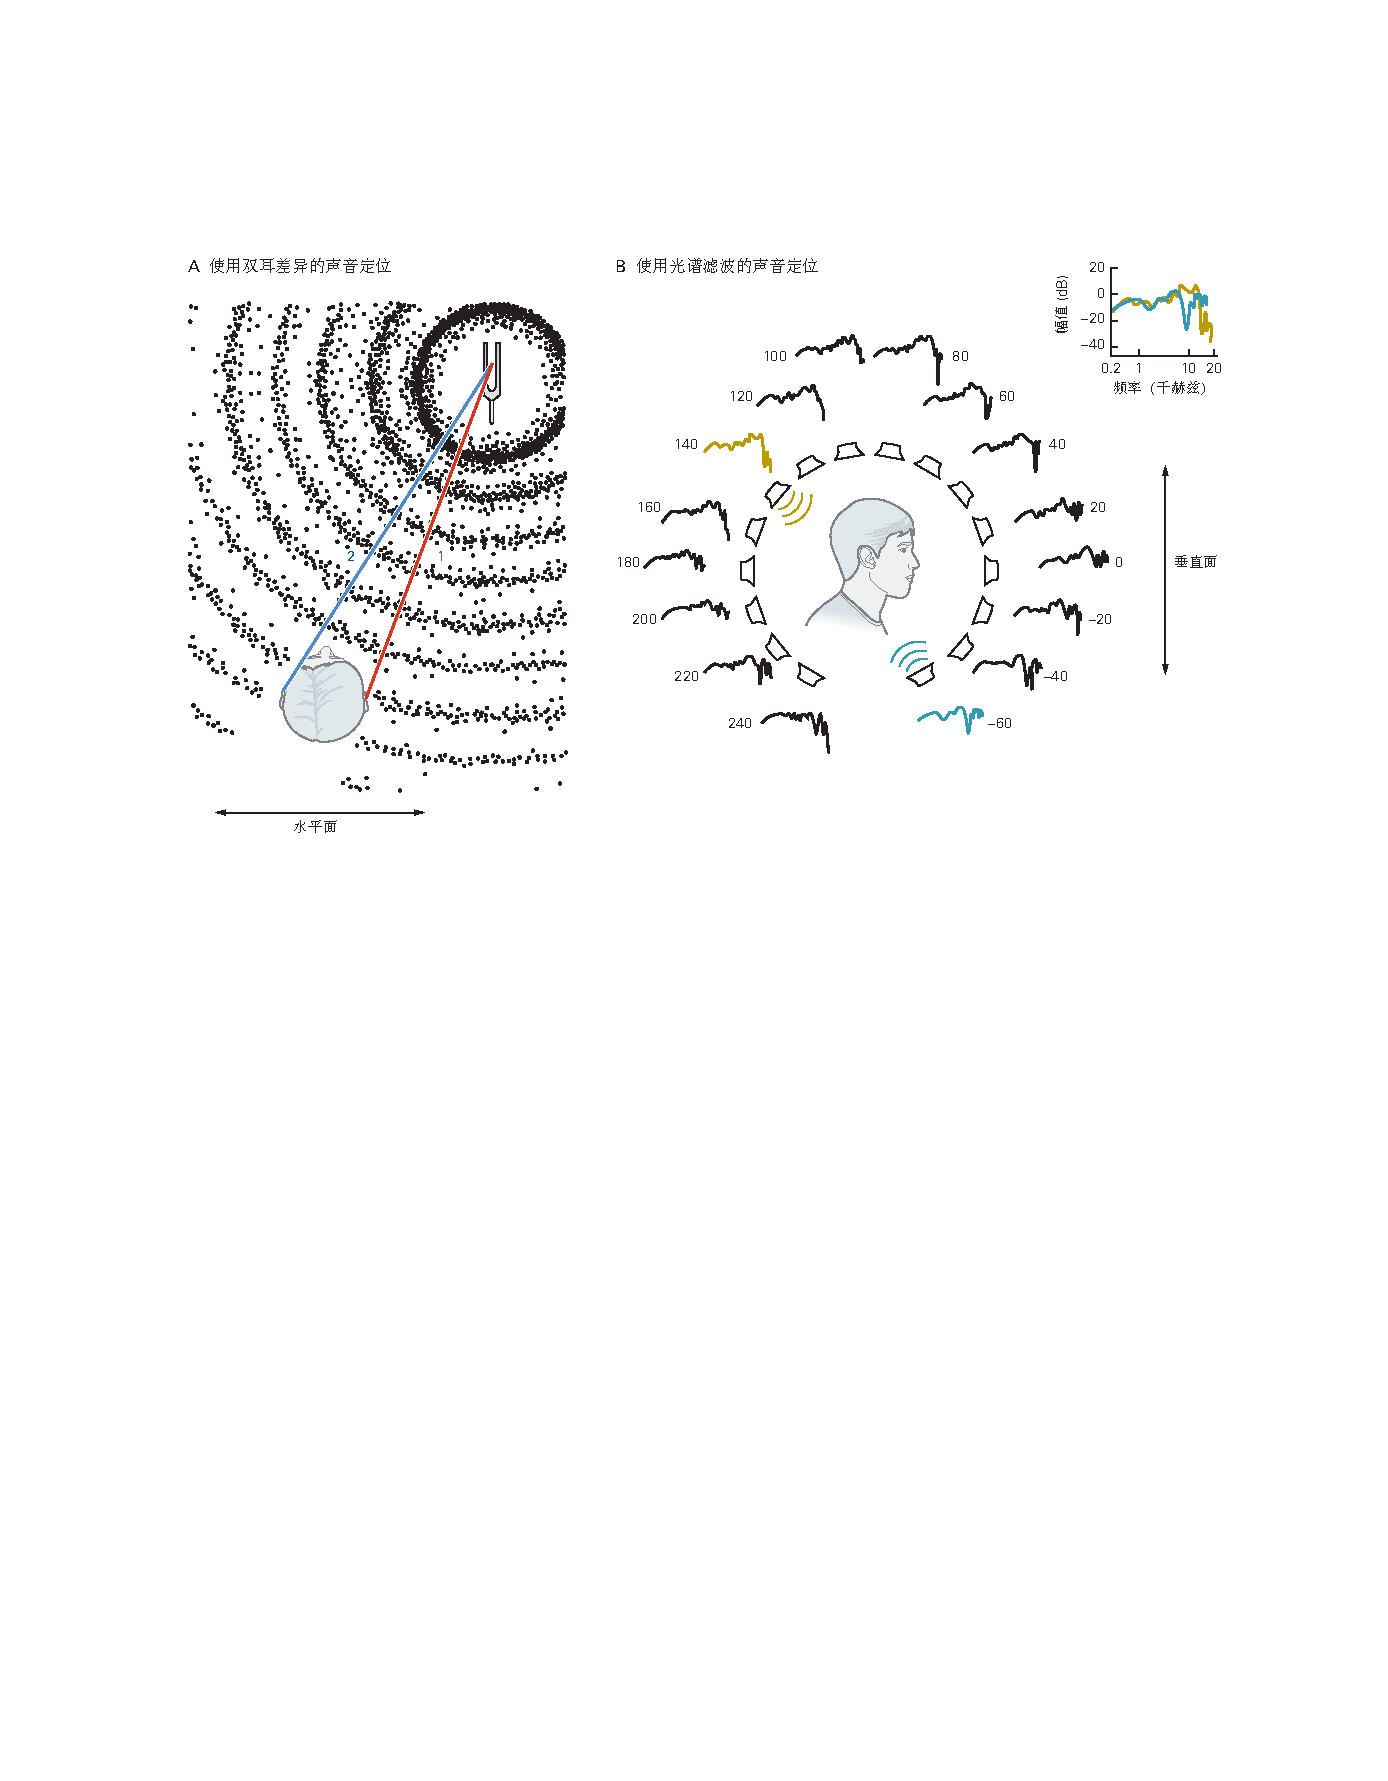
\includegraphics[width=1.0\linewidth]{chap28/fig_28_1}
	\caption*{在水平面上定位声源的提示。
		
	A. 双耳时间和强度差异是在水平面或方位角定位声源的线索。 在水平面上发出的声音到达两只耳朵的方式不同:声音到达的时间较早,并且越靠近声源的耳朵声音越大。 直接从前方或后方发出的声音到达左右耳的距离相同,因此同时到达双耳。 耳间时间和强度不随垂直平面中声源的移动而变化,因此不可能在垂直平面中定位纯正弦音调。 在人类中,最大的耳间时间差约为 600 微秒。 波长短的高频声音被头部偏转,在远处产生声影。 (经许可改编自 Geisler 1998。)

	B. 哺乳动物可以在频谱过滤的基础上在垂直和水平平面上定位宽带声音。 当通过扬声器呈现在人类听觉范围内的所有频率上都具有相同能量的噪声(白噪声)时,耳朵、头部和肩部会抵消某些频率的能量并增强其他频率的能量。 从扬声器发出的白噪声具有平坦的功率谱,但当噪声到达耳道底部时,其频谱不再平坦。

	在图中,耳膜处每个频率的声能相对于白噪声的声能由每个扬声器旁边的轨迹显示; 这些轨迹绘制了以分贝为单位的相对声音幅度与频谱频率(与头部相关的传递函数)的关系。 右上角的小图比较了两种与头部相关的传递函数:一种是针对听者前方出现的低噪声(蓝色),另一种是针对来自听者脑后的噪声(棕色)。 与头部相关的传递函数在大于 8 kHz 的频率处具有深陷波,其频率因声音的产生位置而异。 高频和窄带声音缺乏能量的声音很难在垂直平面上定位。 由于光谱过滤在水平面上也会发生变化,因此它为一只耳朵失去听力的动物提供了唯一的位置提示。

	您可以通过一个简单的实验来测试这些光谱线索的显着性。 闭上你的眼睛,当朋友在不同的高度直接在你面前叮当作响。 比较您在正常条件下定位声音的能力,以及当您通过用手指从后面推动双耳来扭曲双耳形状时的能力。 (数据来自 D. Kistler 和 F. Wightman。)}
	\label{fig:localizing}
\end{figure}

头部的大小决定了耳间时间延迟与声源位置的关系; 神经元回路决定带时间延迟解析的精度。 由于气压波在空气中的传播速度约为 340 m/s,因此人类的最大耳间延迟约为 600 μs; 在小型鸟类中,最大延迟仅为 35 微秒。 人类可以将正前方声源的位置分辨到大约 1 度以内,对应于 10 微秒的耳间时间差。 编码相对较低频率的神经元特别能很好地传达双耳时间差异。 这些神经元可以在声音的每个周期中的相同位置发射,并以这种方式将耳间时间差编码为耳间相位差。 高频声音会在两只耳朵之间产生声影或强度差异。 对于许多头部较小的哺乳动物来说,高频声音是在水平面上定位声音的主要线索。

哺乳动物可以使用频谱滤波在垂直平面和单耳中定位声音。 高频声音的波长接近或小于头部、肩部和外耳的尺寸,与身体的这些部位相互作用产生相长和相消的干扰,引入宽谱峰和深而窄的谱槽,其频率 随声音的位置而变化(图 28-1B)。 来自不同来源的高频声音被不同地过滤,因为在哺乳动物中,外耳的形状从后到前以及从上到下不同。 动物学会使用这些光谱线索来定位声源。 如果通过实验改变耳朵的形状,即使是成年人也可以学会使用新的光谱线索模式。 如果动物的一只耳朵失去听力,它们就会失去耳间时间和强度线索,并且必须完全依赖光谱线索来定位声音。

我们如何理解我们听到的复杂多变的声音? 大多数自然声音都包含广泛频率范围内的能量,并随时间迅速变化。 用于识别声音的信息因动物种类而异,并且取决于聆听条件和经验。 例如,人类的语言可以在噪音中、通过扭曲声音的电子设备甚至通过人工耳蜗来理解。 其稳健性的一个原因是语音包含冗余线索:发声器官产生的声音中有多个参数是共变的。 与此同时,这使得理解动物如何识别模式成为一项复杂的任务。 目前尚不清楚动物在不同条件下会使用哪些线索。

音乐是人类快乐的源泉。 乐器和人声产生的声音在对应于其感知音高的基频以及该频率的倍数处具有能量,赋予声音一种质量,例如,当他们使用时,我们可以区分长笛和小提琴 音高是一样的。 音调主要在低频范围内,听觉神经纤维在这个范围内与声音同相发射。 在音乐中,声音同时组合产生和弦,并相继产生旋律。 悦耳、悦耳的和弦会在耳蜗神经纤维中引起规律、周期性的放电。 在不和谐的声音中,声音本身和听觉神经纤维的放电都不太规律; 分量频率非常接近,以至于它们相互干扰而不是周期性地相互增强。


\section{中央通路中声音的神经表征始于耳蜗核}
处理声学信息的神经通路从耳朵延伸到脑干,通过中脑和丘脑,到达大脑皮层(图 28-2)。 声学信息从耳蜗神经节中的细胞(见图 26-17)传送到脑干中的耳蜗核。 这些信息由几种不同类型的神经元接收,其中大多数神经元按音调排列。

\begin{figure}[htbp]
	\centering
	\includegraphics[width=1.0\linewidth]{chap28/fig_28_2}
	\caption*{中枢听觉通路从脑干通过中脑和丘脑延伸到听觉皮层。 耳蜗神经(颅神经 VIII)中的纤维终止于脑干的耳蜗核。 这些细胞核的神经元通过几条平行通路投射到下丘。 它们的轴突通过梯形体、中间听纹或背侧听纹退出。 一些细胞直接终止于下丘。 其他接触上橄榄复合体和外侧丘系细胞核中的细胞,后者又投射到下丘。 下丘的神经元投射到上丘和丘脑的内侧膝状体核。 丘脑神经元投射到听觉皮层。 耳蜗核和外侧丘系的腹侧核是唯一接收单耳输入的中枢听觉神经元。}
	\label{auditory_pathways}
\end{figure}

不同类型神经元的轴突采用不同的路径到达脑干和中脑,并在不同的目标处终止。 从耳蜗核到对侧下丘的一些通路是直接的; 其他涉及脑干听觉核中的一个或两个突触阶段。 从双侧下丘,声音信息以两种方式流动:到同侧上丘,在那里它参与调整头部和眼睛对声音的反应,以及到同侧丘脑,传递到大脑皮层的听觉区域。 从外围到更高脑区的传入听觉通路包括许多级别的传出反馈。

\subsection{耳蜗神经以平行途径将声学信息传递到音调组织的耳蜗核}
来自耳蜗神经节细胞的传入神经纤维被束缚在耳蜗或前庭耳蜗神经(脑神经 VIII)的听觉成分中,并完全终止于耳蜗核。 哺乳动物的耳蜗神经包含两组纤维:大量 (95\%) 的有髓纤维接收来自内毛细胞的输入,以及少量 (5\%) 的无髓纤维接收来自外毛细胞的输入。

与无髓纤维相比,更大、更多的有髓纤维更容易被理解。 每种类型都检测狭窄频率范围内的能量; 因此,耳蜗神经纤维的音调阵列携带着关于声音频率内容如何随时间变化的详细信息。 无髓神经纤维既终止于耳蜗腹侧核的大神经元,也终止于耳蜗腹侧核周围的小颗粒细胞。 因为很难从这些细小的纤维中记录下来,所以它们传递给大脑的信息还没有被很好地理解。 无髓神经纤维整合来自耳蜗相对广泛区域的信息,但对声音没有反应。 有人提出,这些纤维对耳蜗损伤有反应,并会导致听觉过敏——接触会损伤耳蜗的响亮声音后会感到疼痛。

耳蜗核的两个特征很重要。 首先,这些原子核按同位素组织。 携带来自检测低频的耳蜗顶端信息的纤维在腹侧和背侧耳蜗核的腹侧终止; 那些从检测高频的耳蜗基端携带信息的那些,在背侧终止(图 28-3)。 其次,每个耳蜗神经纤维支配耳蜗核内的几个不同区域,将具有不同投射模式的各种类型的神经元联系到更高的听觉中枢。 因此,听觉通路包括至少四个平行的上升通路,它们同时从耳蜗神经纤维携带的信号中提取不同的声学信息。 并联电路是脊椎动物感觉系统的一般特征。



\subsection{耳蜗腹核提取有关声音的时间和频谱信息}
无层腹侧耳蜗核的主要细胞可锐化时间和光谱信息,并将其传送到听觉通路的更高中心。 三种类型的神经元混合在一起,并通过脑干形成不同的通路(图 28-4)。

浓密细胞双侧投射到上橄榄复合体。 这条路有两部分。 一个穿过内侧上橄榄并比较声音到达两只耳朵的时间; 另一个穿过梯形体的内侧核和外侧上橄榄并比较耳间强度。 大的球形浓密细胞感知低频并双侧投射到内侧上橄榄,形成检测耳间时间延迟并有助于水平面低频声音定位的电路。 小球形浓密细胞和球状浓密细胞感知更高的频率。 小球形浓密细胞刺激同侧外侧上橄榄。 球状浓密细胞通过花萼末梢刺激梯形体对侧内侧核中的神经元,进而抑制外侧上橄榄的主要细胞。 外侧上橄榄中的神经元整合了同侧兴奋和对侧抑制,以测量耳间强度并定位水平面中的高频声音源(见图 28-6)。

星状细胞广泛终止。 它们兴奋同侧耳蜗背核的神经元,梯形体腹核中的内侧橄榄蜗传出神经元,同侧外侧上橄榄附近的橄榄周核,以及外侧丘系,下丘的对侧腹核, 和丘脑。 星状细胞的同位素阵列对声音的频谱进行编码。

章鱼细胞激发对侧橄榄旁核中的靶标,并终止于外侧丘系腹侧核神经元上的大兴奋性肾盏末梢,这反过来又对下丘提供了及时的甘氨酸能抑制。 章鱼细胞检测声音的开始,使动物能够检测到短暂的间隙。 它们标记来自一个来源的光谱成分,这些成分必须一起开始。

这些通路通过腹侧耳蜗核执行的综合任务的差异反映在细胞形态上。 它们的树突形状反映了它们从耳蜗神经纤维收集信息的方式。 高度调谐的浓密和星状细胞的树突从相对较少的耳蜗神经纤维接收输入,而相比之下,广泛调谐的章鱼细胞的树突垂直于耳蜗神经纤维的路径,准备接收来自许多耳蜗神经纤维的输入 . 浓密细胞的许多输入来自包裹浓密细胞体的异常大的终端,满足它们对大突触电流的需要。 章鱼细胞对大突触电流的需求是通过对来自大量小终端的输入求和来满足的。

神经元的生物物理学特性决定了突触电流如何转化为电压变化,以及突触输入被整合的时间长短。 腹侧耳蜗核中的章鱼和浓密细胞能够以异常快速和精确定时的突触电位做出反应。 这些神经元具有显着的低电压激活 K+ 电导,可提供低输入电阻和快速响应并防止重复放电(图 28–4C)。 在这些渗漏细胞中触发动作电位所需的大突触电流通过许多突触处的快速门控、高电导、AMPA 型(α-氨基-3-羟基-5-甲基异恶唑-4-丙酸盐)谷氨酸受体传递 发布网站。 相比之下,即使相对较小的去极化电流也会产生较大的持续电压变化的星状细胞会响应突触电流而产生较慢的兴奋性突触后电位 (EPSP),而 N-甲基-d-天冬氨酸 (NMDA) 型谷氨酸受体会增强这些响应。


\subsection{耳蜗背核将声学与体感信息相结合,利用频谱线索定位声音}

在脊椎动物中,只有哺乳动物具有背侧耳蜗核。 耳蜗背核接收来自投射到不同层的两个神经元系统的输入(图 28–4A、B)。 它的主要细胞梭形细胞整合了这两个输入系统,并将结果直接传送到对侧下丘。

最外层的分子层是平行纤维系统的末端,颗粒细胞的无髓鞘轴突散布在耳蜗核内和周围。 该系统将体感、前庭和听觉信息从大脑的广泛区域传输到分子层。

深层接收声音信息。 不仅耳蜗神经纤维而且腹侧耳蜗核的星状细胞也终止于深层。 声学输入按音调分布在与平行纤维成直角的等频层中。

梭形细胞是耳蜗背核的主要细胞,整合了两个输入系统。 分子层中的平行纤维通过分子层顶端树突上的刺激发梭形细胞。 平行纤维也终止于车轮细胞的树突棘,中间神经元与小脑浦肯野细胞非常相似,后者反过来抑制梭状细胞。 腹侧耳蜗核中的耳蜗神经纤维和星状细胞通过深层光滑基底树突上的突触激发梭状细胞和抑制性中间神经元。

最近的实验表明,耳蜗背核的回路可以区分不可预测和可预测的声音。 例如,动物自己的咀嚼或舔舐声音是可以预测的,并通过这些电路消除。 当动物移动头部、耳朵或肩膀时出现的光谱线索变化,改变了声音入射到耳朵的角度,这是不可预测的,尤其是当外部声源移动时。 关于头部和耳朵位置的体感和前庭信息,以及来自更高层次神经系统的关于动物自身运动的下行信息,通过分子层调制到达深层的声学信息。

\section{哺乳动物的上橄榄复合体包含用于检测耳间时间和强度差异的独立电路}
在许多脊椎动物中,包括哺乳动物和鸟类,上橄榄复合体中的神经元比较双侧耳蜗核中细胞的活动以定位声源。 单独的电路检测耳间时间和强度差异并投射到下丘。

\subsection{内侧上橄榄生成耳间时差图}
到达耳朵的时间差异不会在耳蜗中表现出来。 相反,它们首先出现在内侧上橄榄中,通过比较两耳声音反应中动作电位的时间来创建耳间相位图。 声音在到达远耳之前先到达近耳,双耳时间差与声源在水平面上的位置直接相关(图 28-5A)。

调谐到 4 kHz 以下频率的耳蜗神经纤维及其浓密的细胞目标通过与压力波同相发射来编码声音。 此属性称为锁相。 尽管单个神经元可能无法在某些周期内放电,但某些神经元组会在每个周期内放电。 在这样做的过程中,这些神经元携带有关声音每个周期的输入时间的信息。 从一侧到达的声音会引起锁相发射,这种发射在近耳处始终比在远耳处更早,从而导致一致的耳间相位差(图 28-5A)。


1948 年,Lloyd Jeffress 提出,来自两只耳朵的重合输入的检测器阵列,通过由具有系统不同长度的轴突组成的延迟线传输,可以形成耳间时间差异图,从而形成声源位置图( 图 28-5B)。 在这样的电路中,传导延迟补偿了较早到达近耳的情况。 随着声音从中线移动到侧面,双耳时间延迟系统地增加,导致向神经元阵列的边缘进一步同步发射。

此类神经元图谱已在谷仓猫头鹰的内侧上橄榄核同系物中发现。 哺乳动物和鸡使用这种输入排列的变体。 内侧上橄榄的主要神经元在中线的每一侧形成一个或几个细胞厚度的薄片。 每个神经元有两簇树突,一个延伸到薄片的侧面,另一个延伸到薄片的内侧(图 28-5C)。 侧面的树突与来自同侧耳蜗核的大球形浓密细胞的轴突接触,而内侧的树突与来自对侧耳蜗核的匹配最佳频率的大球形浓密细胞接触。 正如 Jeffress 所建议的那样,浓密细胞的轴突终止于具有延迟线的对侧内侧上橄榄,但终止于同侧内侧上橄榄的分支长度相等(参见图 28-5C)。

传导延迟使得每个内侧上橄榄只有在声音来自对侧一半空间时才会从两只耳朵接收一致的兴奋性输入。 当声源从中线移动到头部对侧的最外侧点时,声音较早到达对侧耳朵需要通过连续更长的延迟线来补偿。 这导致来自两只耳朵的输入在内侧上橄榄的连续更多的后部和外侧区域重合。 叠加在这些兴奋性输入上的抑制在锐化耳间相位图方面起着重要作用。

在编码耳间相位时,内侧上橄榄中的单个神经元提供关于耳间时间差异的模糊信息。 当声音具有多个频率的能量时,相位模糊就会得到解决,自然声音几乎总是如此。 内侧上橄榄的神经元片形成沿 rostrocaudal 和后内侧维度的耳间阶段的表示。 浓密细胞输入的阵列也在背腹维度强加了一个同位素组织。 包含多个频率能量的声音会在单个背腹侧神经元列中引起最大同步放电,从而明确定位声源。 使用耳间相位来编码耳间时间差异的美妙之处在于,大脑不仅在声音的开始和结束时而且在持续声音的每个周期中都接收到有关耳间时间差异的信息。

内侧上橄榄的主要细胞也受到来自同侧和对侧的声音分别通过斜方体的外侧核和内侧核的急剧定时抑制。 值得注意的是,尽管抑制是通过具有额外突触的通路介导的,但通过来自两侧的通路的抑制作用先于兴奋的到来,并加剧了兴奋的总和。 球状浓密细胞的大轴突和 Held 的大肾盏末端使得通过梯形体内侧核的突触通路的高传导速度成为可能,它们以短而一致的时间激活梯形体内侧核中的神经元 延误。 通过斜方体外侧核带来同侧抑制的途径不太清楚。

因此,每个内侧上橄榄形成了对侧半视野中声源位置的地图。 这种刺激的空间表征与其他感觉系统中的刺激的空间表征之间的显着区别在于,它不是输入空间排列的结果,如视网膜专题图或体感图,而是大脑根据传入通路中的计算推断出来的。


\subsection{外侧上橄榄检测耳间强度差异}
波长与头部相似或小于头部的声音被头部偏转,导致近耳处的强度大于远耳处的强度。 在人类中,耳间强度在频率大于约 2 kHz 的声音中可能会有所不同。 由这种头部阴影产生的耳间强度差异由包括梯形体内侧核和外侧上橄榄的神经元回路检测。

虽然外侧上橄榄不形成声音在水平面上的位置图,但它执行几个综合步骤中的第一步,这些步骤使用耳间强度差异来定位声音。 该核中的神经元平衡同侧兴奋与对侧抑制。 兴奋来自同侧腹侧耳蜗核中的小球形浓密细胞和星状细胞。 抑制来自突触通路,包括对侧耳蜗腹侧核中的球状浓密细胞和梯形体同侧内侧核的主要神经元(图 28-6A)。 同侧出现的声音产生相对强烈的兴奋和相对较弱的抑制,而对侧产生的声音产生比兴奋更强的抑制。 来自同侧半野的声音比来自对侧半野的声音更强烈地激活外侧上橄榄中的神经元。 外侧上橄榄神经元的放电是声源位置的函数,因此携带有关声音在水平面上出现位置的信息(图 28-6B)。

为了平衡一种声音刺激的兴奋和抑制,同侧兴奋和对侧抑制必须同时到达外侧上橄榄的神经元。 因此,从同侧腹侧耳蜗核单突触产生的兴奋必须与从对侧腹侧耳蜗核非突触产生的抑制同时到达。 抑制来自梯形体的内侧核,其输入通过球状浓密细胞的大轴突和 Held 的大花萼产生突触反应,具有短暂且一致的定时延迟。 携带同侧兴奋的小球形浓密细胞和星状细胞的轴突比球状浓密细胞的轴突传导得更慢。

球状浓密细胞的末端,即 Held 的花萼,如此显着地吞没了梯形体神经元的细胞体,以至于它们引起了早期解剖学家和现代生物物理学家的注意。 单个体细胞末端在许多释放位点释放神经递质并产生大的突触电流。 该突触的突触前和突触后记录的可靠性使该站点成为详细研究突触传递机制的理想场所(第 15 章)。


\subsection{上橄榄复合体向耳蜗提供反馈}
虽然感觉系统在很大程度上是传入的,将感觉信息带到大脑,但最近的研究使人们认识到传出信号在听觉系统的许多层面上的重要性。 橄榄蜗神经元形成从上橄榄复合体到耳蜗毛细胞的反馈回路。 它们的细胞体位于橄榄核中主要致密的细胞体簇周围。 在哺乳动物中,两组橄榄耳蜗神经元已在功能上有所区别。 内侧橄榄耳蜗神经元的轴突终止于双侧外毛细胞; 外侧橄榄蜗神经元轴突同侧终止于与内毛细胞相关的传入纤维。

大多数内侧橄榄耳蜗神经元的细胞体位于橄榄复合体的腹侧和内侧,将它们的轴突发送到对侧耳蜗(图 28-7),但许多神经元也投射到同侧耳蜗。 这些胆碱能神经元通过一类特殊的由 α9 和 α10 亚基形成的烟碱乙酰胆碱受体通道作用于毛细胞。 Ca2+ 通过这些通道流入导致 K+ 通道打开,使外毛细胞超极化。 因此,这些神经元调节调谐的负反馈并且是双耳的,主要但不完全由对侧腹侧耳蜗核的星状细胞驱动。 这些传出纤维的活动降低了耳蜗的敏感性,并保护它免受响亮声音的损害。 内侧橄榄耳蜗神经元的侧支终止于耳蜗核中的星状细胞,作用于传统的烟碱和毒蕈碱乙酰胆碱受体,形成兴奋性反馈回路。

外侧橄榄耳蜗神经元的细胞体位于外侧上橄榄体内和周围,将它们的轴突专门发送到同侧耳蜗,在那里它们终止于来自内毛细胞的传入纤维。 查尔斯·利伯曼 (Charles Liberman) 和他的同事证明,这些传出神经可以平衡两只耳朵的耳蜗神经纤维的兴奋性。



\subsection{下丘外侧丘系形状响应的腹侧核和背侧核抑制}
来自耳蜗和上橄榄核的纤维在从脑干上升到下丘时沿着大脑的外侧边缘呈带状或丘系分布。 沿着这条纤维带的是神经元组,它们形成了外侧丘系的背核和腹核。 外侧丘系腹侧核中的神经元接收来自腹侧耳蜗核所有主要细胞群的输入,主要对由对侧耳驱动的单耳输入作出反应,而背侧核中的神经元接收来自外侧和内侧上级的输入 橄榄核并对来自双耳的输入做出反应。 两个分支中的神经元都具有抑制作用并投射到下丘。 他们的角色很有趣,但还没有被完全理解。

由于失去一只耳朵不会大大影响对声音含义的理解,因此外侧丘系腹侧核的主要单声道功能涉及声音含义的处理是有道理的。 此外,哺乳动物从其声学环境中提取的信息各不相同,这可能解释了不同物种在外侧丘系腹侧核的结构和功能方面的差异。

一些哺乳动物物种比其他物种更明显的边界将腹核和中间核以及外侧丘系的腹核的细分分开。 神经元的形状、生物物理特性和耳蜗核输入的收敛模式各不相同。 一组甘氨酸能神经元受来自章鱼细胞的大肾盏末梢支配。 这些可以在下丘产生抑制性时间参考信号。 一些广泛调谐的神经元几乎完全在音调开始时放电,具有敏锐的定时动作电位,但在复杂的声音中传达周期性,提出了这些神经元是否可能在编码音乐和语音的音调中起作用的问题。 只要有提示音,其他人就会开火; 这些神经元跟踪强度的波动或声音的包络,这一特征有助于理解包括语音在内的声音的含义。 神经元的调谐曲线是可变的,许多是宽的或 W 形的。

背核中的神经元主要是双耳神经元,接收来自同侧内侧上橄榄和外侧上橄榄的输入,主要来自对侧。 这些神经元是 GABAergic,靶向两侧的下丘,也靶向外侧丘系的对侧背核。 背核神经元的兴奋被 NMDA 型谷氨酸受体放大,因此它们在目标中产生的抑制比声音刺激持续数十毫秒,因此被称为持续抑制。 为了准确定位声音,动物必须忽略在初始直达波阵面之后到达的周围表面的声音反射。 心理物理学实验表明,哺乳动物会抑制除最先到达的声音以外的所有声音,这种现象称为优先效应。 已经提出,来自外侧丘系背核的下丘的持续抑制用于抑制虚假定位线索,例如回声,因此它有助于优先效应。


\section{传入听觉通路在下丘汇聚}
下丘在所有脊椎动物的听觉通路中占据中心位置,因为所有上行通过脑干的听觉通路都汇聚于此(图 28-7)。 最重要的激发源是对侧耳蜗腹核的星状细胞、对侧耳蜗背核的梭形细胞、同侧内侧上橄榄和对侧外侧上橄榄的主要细胞、同侧和对侧耳蜗背核的主要细胞。 侧丘系、对侧下丘的连合连接和听觉皮层 V 层的锥体细胞。 重要的抑制源包括外侧丘系、同侧外侧上橄榄核、上橄榄旁核和对侧下丘。

哺乳动物的下丘分为中央核、背侧皮质和外部皮质。 中央核是同位素组织的。 在具有相似最佳频率的椎板中,低频在背外侧表示,高频在腹内侧表示。 精细映射表明同位素组织是不连续的; 最佳频率之间的间隔对应于心理物理学测量的大约三分之一倍频程的临界频带。 尽管中央核按音调组织,但这些神经元的输入频谱范围比听觉通路的早期阶段更广泛。 抑制可以是广泛的并缩小兴奋性神经元的反应。 此外,可以通过降低来自皮层的输入来调制调谐。

中央核中的许多神经元携带有关声源位置的信息。 这些细胞中的大多数对耳间时间和强度差异敏感,这是在水平面上定位声音的基本线索。 神经元也对将声音定位在垂直平面上的频谱线索敏感。 已经在下丘中测量了优先效应的生理相关性,其中抑制抑制了声音的模拟反射。

% 原文中这一段和下一节重复了


\subsection{来自下丘的声音位置信息在上丘中创建声音的空间图}
下丘不仅是会聚点,也是上升或流出通路的分支点。 中央核的神经元投射到下丘的外部皮层,也投射到丘脑和下丘臂的核,然后两者都投射到上丘(或鸟类的视顶盖)。

上丘对于头部和眼睛对空间中的听觉和视觉线索的反射性定向运动至关重要。 当作为哺乳动物声音定位基础的双耳声音线索和单耳频谱线索到达上丘时,它们已被合并以创建声音的空间图,其中神经元明确地调整到特定的声音方向。 这种收敛是至关重要的,因为仅凭电平和时间的双耳差异不能明确编码空间中的单个位置。 必须考虑提供有关垂直位置信息的光谱提示,因为垂直平面中的不同位置会在时间或强度上产生相同的耳间差异。 这种明确的空间映射出现在鸟类和一些哺乳动物身上(图 28-8)。 在雪貂和豚鼠中,它发生在外皮层和下丘的臂核中。

在上丘内,听觉地图与视觉空间和身体表面的地图对齐。 与视觉和体感空间图不同,听觉空间图不反映周围感受器表面; 相反,它是根据识别声源在空间中的特定位置的线索组合计算得出的。

上丘中的听觉、视觉和体感神经元都汇聚在同一结构的输出通路上,该结构控制眼睛、头部和外耳的定向运动。 上丘的运动回路相对于空间中的运动目标进行映射,并与感觉映射对齐。 这种感觉-运动对应有助于运动的感觉引导。



\section{下丘传输声音信息给大脑皮层}
听觉信息从下丘上升到丘脑的内侧膝状体,然后从那里到达听觉皮层。 
来自下丘的通路包括丘系或核心通路和丘脑外或带状通路。 
从听觉皮层到内侧膝状体的下降投射在解剖学和功能上都很突出。

\subsection{沿着上行通路刺激选择性逐渐增加}
沿着上升通路的结构中听觉神经元的一个显着特征是它们逐渐增加的刺激选择性。 
听觉神经纤维主要对一个刺激维度具有选择性,即纯音的频率。 
中枢听觉系统神经元的刺激选择性可能是多维的,如频率、频谱带宽、声强、调制频率和空间位置等。 
在这个多维声学空间中,神经元在沿上升通路的连续听觉区域变得更具选择性。

听觉皮层中的许多神经元(尤其是上皮层中的神经元)对声学刺激具有高度选择性,因此神经元的首选(接近最佳)刺激仅占据其在多维声学空间中感受野的一小部分区域。 
在通往听觉皮层的路径上,首选刺激的区域在结构上变得越来越小(图 28-9A)。 
纯音和宽带噪声是广泛声学刺激的两种极端情况,它们可以优先驱动听觉皮层神经元。 
听觉皮层中的大多数神经元优先受具有比纯音和宽带噪声更大的频谱和时间复杂性的刺激驱动。

\begin{figure}[htbp]
	\centering
	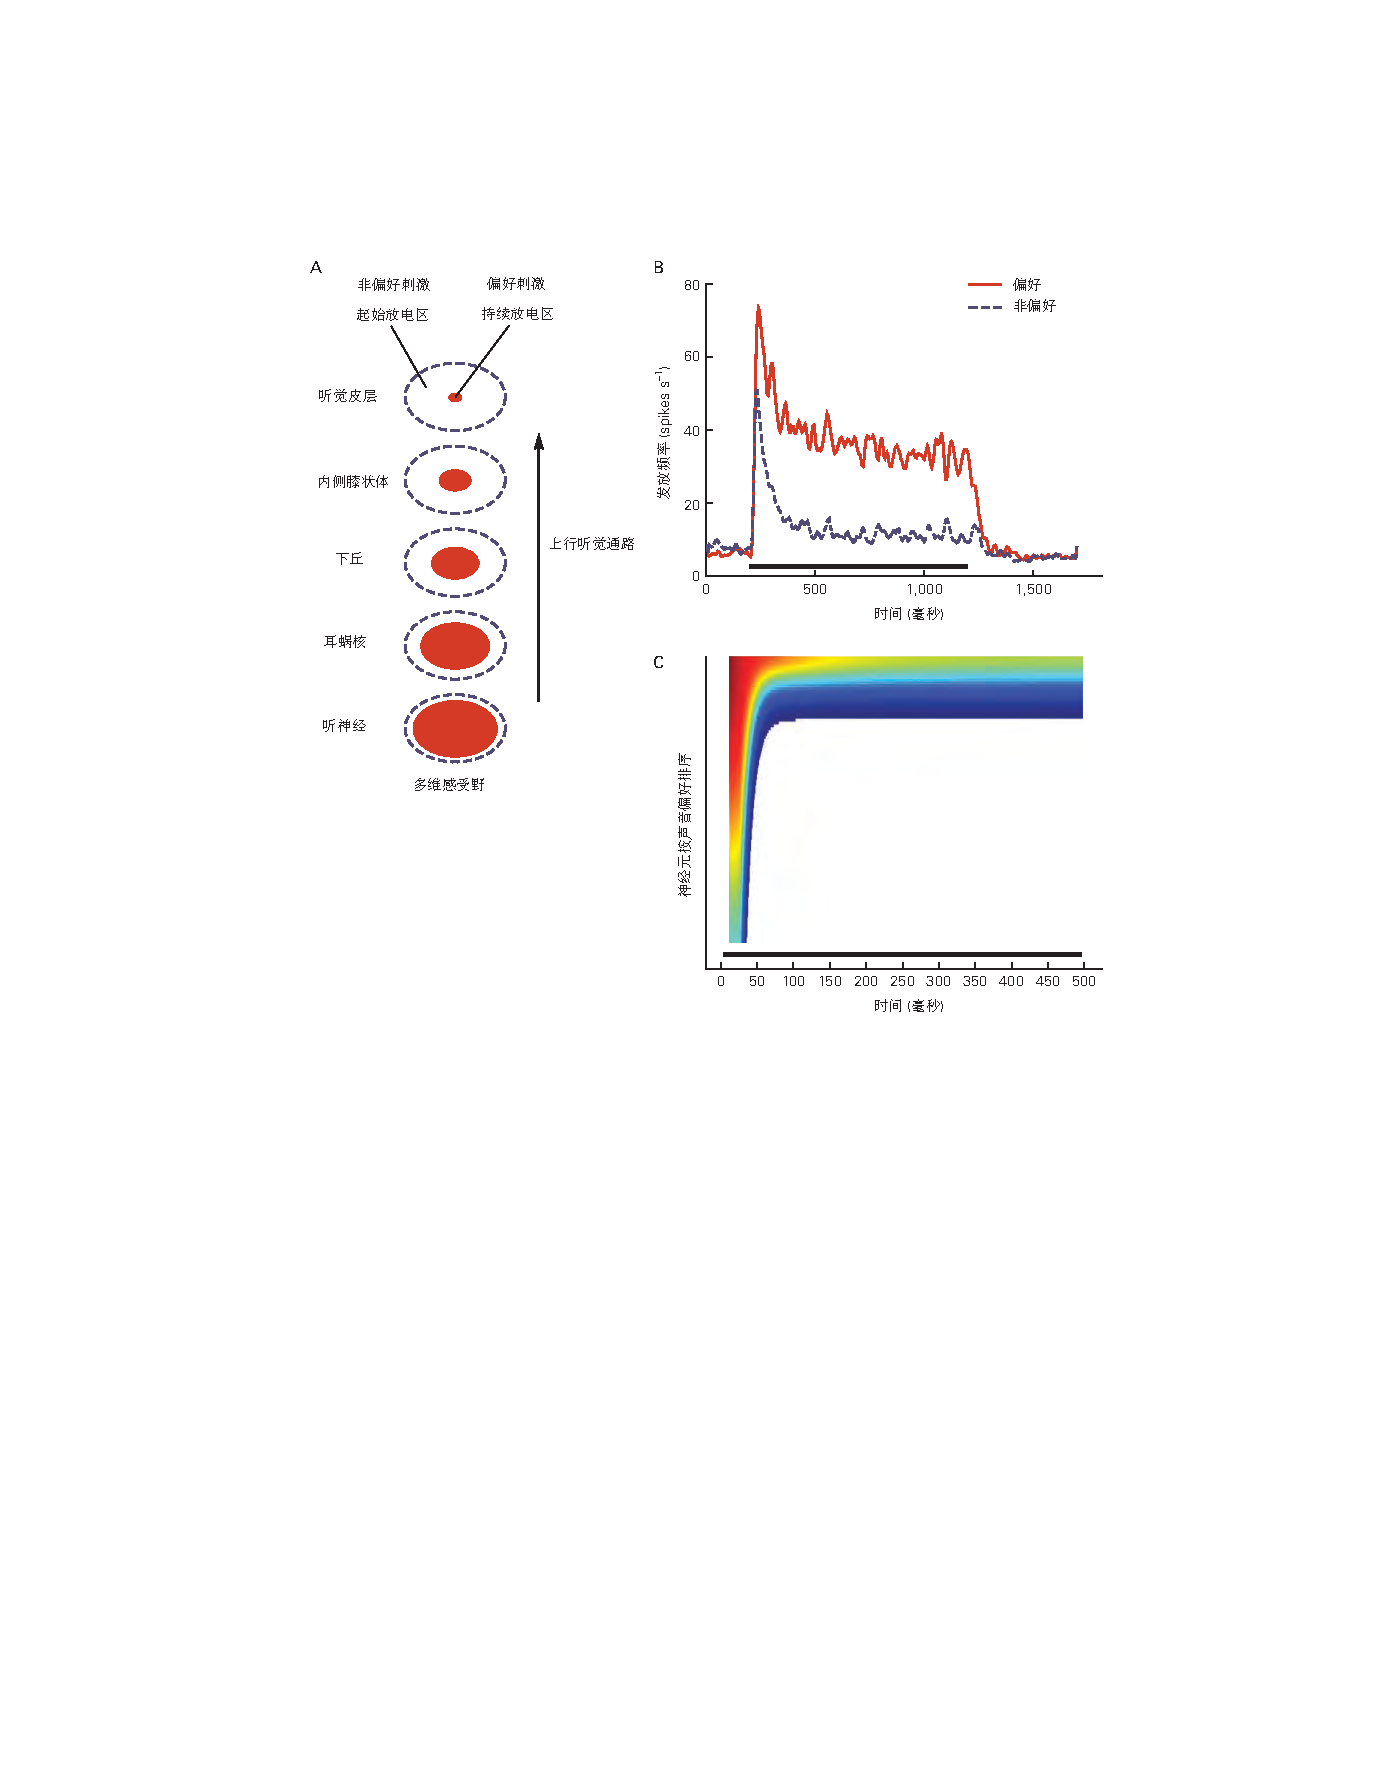
\includegraphics[width=0.5\linewidth]{chap28/fig_28_9}
	\caption{刺激选择性沿上行听觉通路增加。 
		A. 刺激选择性以及沿上行听觉通路的持续放电和起始放电之间的关系。 
		每个空心椭圆代表二维平面上所示神经元的多维感受野 (Receptive Field, RF)。 
		实心椭圆代表神经元 RF 的“持续放电区域”(对应于首选刺激)。 
		RF 内的其余区域是“起始激发区”(对应于非偏好刺激)。 
		神经元表现出持续或开始放电,这取决于 RF 的哪个区域受到刺激。 
		如果刺激落在 RF 之外,神经元就不会发射。 (经许可改编自 Wang 2018。)
		B. 群体平均放电率响应初级听觉皮层 (A1) 中每个神经元的偏好和非偏好刺激。 
		在清醒的狨猴中进行细胞外记录。 粗条 = 刺激持续时间。 
		(经许可改编自 Wang 等人,2005 年。版权所有 © 2005 Springer Nature。)
		C. A1 神经元响应声音爆发的活动分布。 
		在 y 轴上,所有 A1 神经元都根据它们对特定刺激的偏好进行排序。 
		蓝色到红色的颜色渐变表示增加的放电率。 
		具有最高放电率的神经元位于 y 轴的顶端。 黑条 = 刺激持续时间。 
		大多数神经元对声音的开始表现出短暂的相位反应,但只有那些特别适应声音的神经元才会保持反应直到声音结束。 
		(经许可改编自 Middlebrooks 2005。版权所有 © 2005 Springer Nature。)}
	\label{fig:28_9}
\end{figure}

刺激选择性的增加还伴随着神经元放电模式的变化。 
当神经元被它们喜欢的刺激驱动时,它们不仅会以更高的放电率做出反应,而且还会在整个刺激持续时间内持续放电(图\ref{fig:28_9}B)。 
皮层神经元的感受野在较大的“起始放电区”(对应于非偏好刺激)内包含一个“持续放电区”(对应于偏好刺激)。 这
解释了为什么实验者在播放连续声音时通常会观察到听觉皮层的起始(相位)反应。

发现如何在听觉皮层中引发持续放电很重要,因为它提供了神经放电与连续声事件感知之间的直接联系。 
听觉皮层神经元的这种持续放电仅在清醒的动物中观察到。 
相比之下,只要刺激的光谱能量落在神经元的感受野内,无论是在麻醉还是清醒的情况下,听觉神经纤维通常都会对广泛的声信号做出持续的反应。 
半个多世纪前,当 David Hubel 和他的同事冒险进入听觉皮层时,他们对驱动清醒猫的听觉皮层中的神经元有多么困难感到困惑。 
现在我们知道这是因为它们可能是从高度选择性的神经元记录并使用非偏好的刺激。 
从那时起,数字技术的可用性使得创建和测试大量声学刺激成为可能,以寻找听觉皮层中高度选择性神经元的首选刺激。 
实验者阐明的总体情况是,当听到声音时,听觉皮层首先通过相对大量的神经元进行瞬时放电(编码声音的开始)。 
随着时间的流逝,激活变得仅限于优先由声音驱动的较小数量的神经元(图\ref{fig:28_9}C),这导致神经元群体内和随着时间的推移对声音的选择性表示。 
因为每个神经元都有自己的偏好刺激,不同于其他神经元的偏好刺激,听觉皮层中的神经元以其持续放电区共同覆盖整个听觉空间。 
因此,任何特定的声音都可以在听觉皮层的特定神经元群中激发整个持续时间的持续放电。 
换句话说,在全脑成像(例如,功能性磁共振成像 [fMRI]、正电子发射断层扫描 [PET])中被声刺激激活的听觉皮层区域包含优先由声刺激驱动的神经元。


\subsection{听觉皮层映射众多的声音层面}
听觉皮层包括位于颞叶背面的多个不同功能区域。 
最明显的投射是从内侧膝状体的腹侧部到初级听觉皮层(A1,或 Brodmann 区 41)。 
与皮质下结构一样,这个细胞结构不同区域中的神经元按同位素排列。 
在猴子中,调谐到低频的神经元位于 A1 的喙端,而那些对高频敏感的神经元位于尾部区域(图\ref{fig:28_10})。 
因此,就像视觉和体感皮层一样,A1 包含反映感觉外围的地图。

\begin{figure}[htbp]
	\centering
	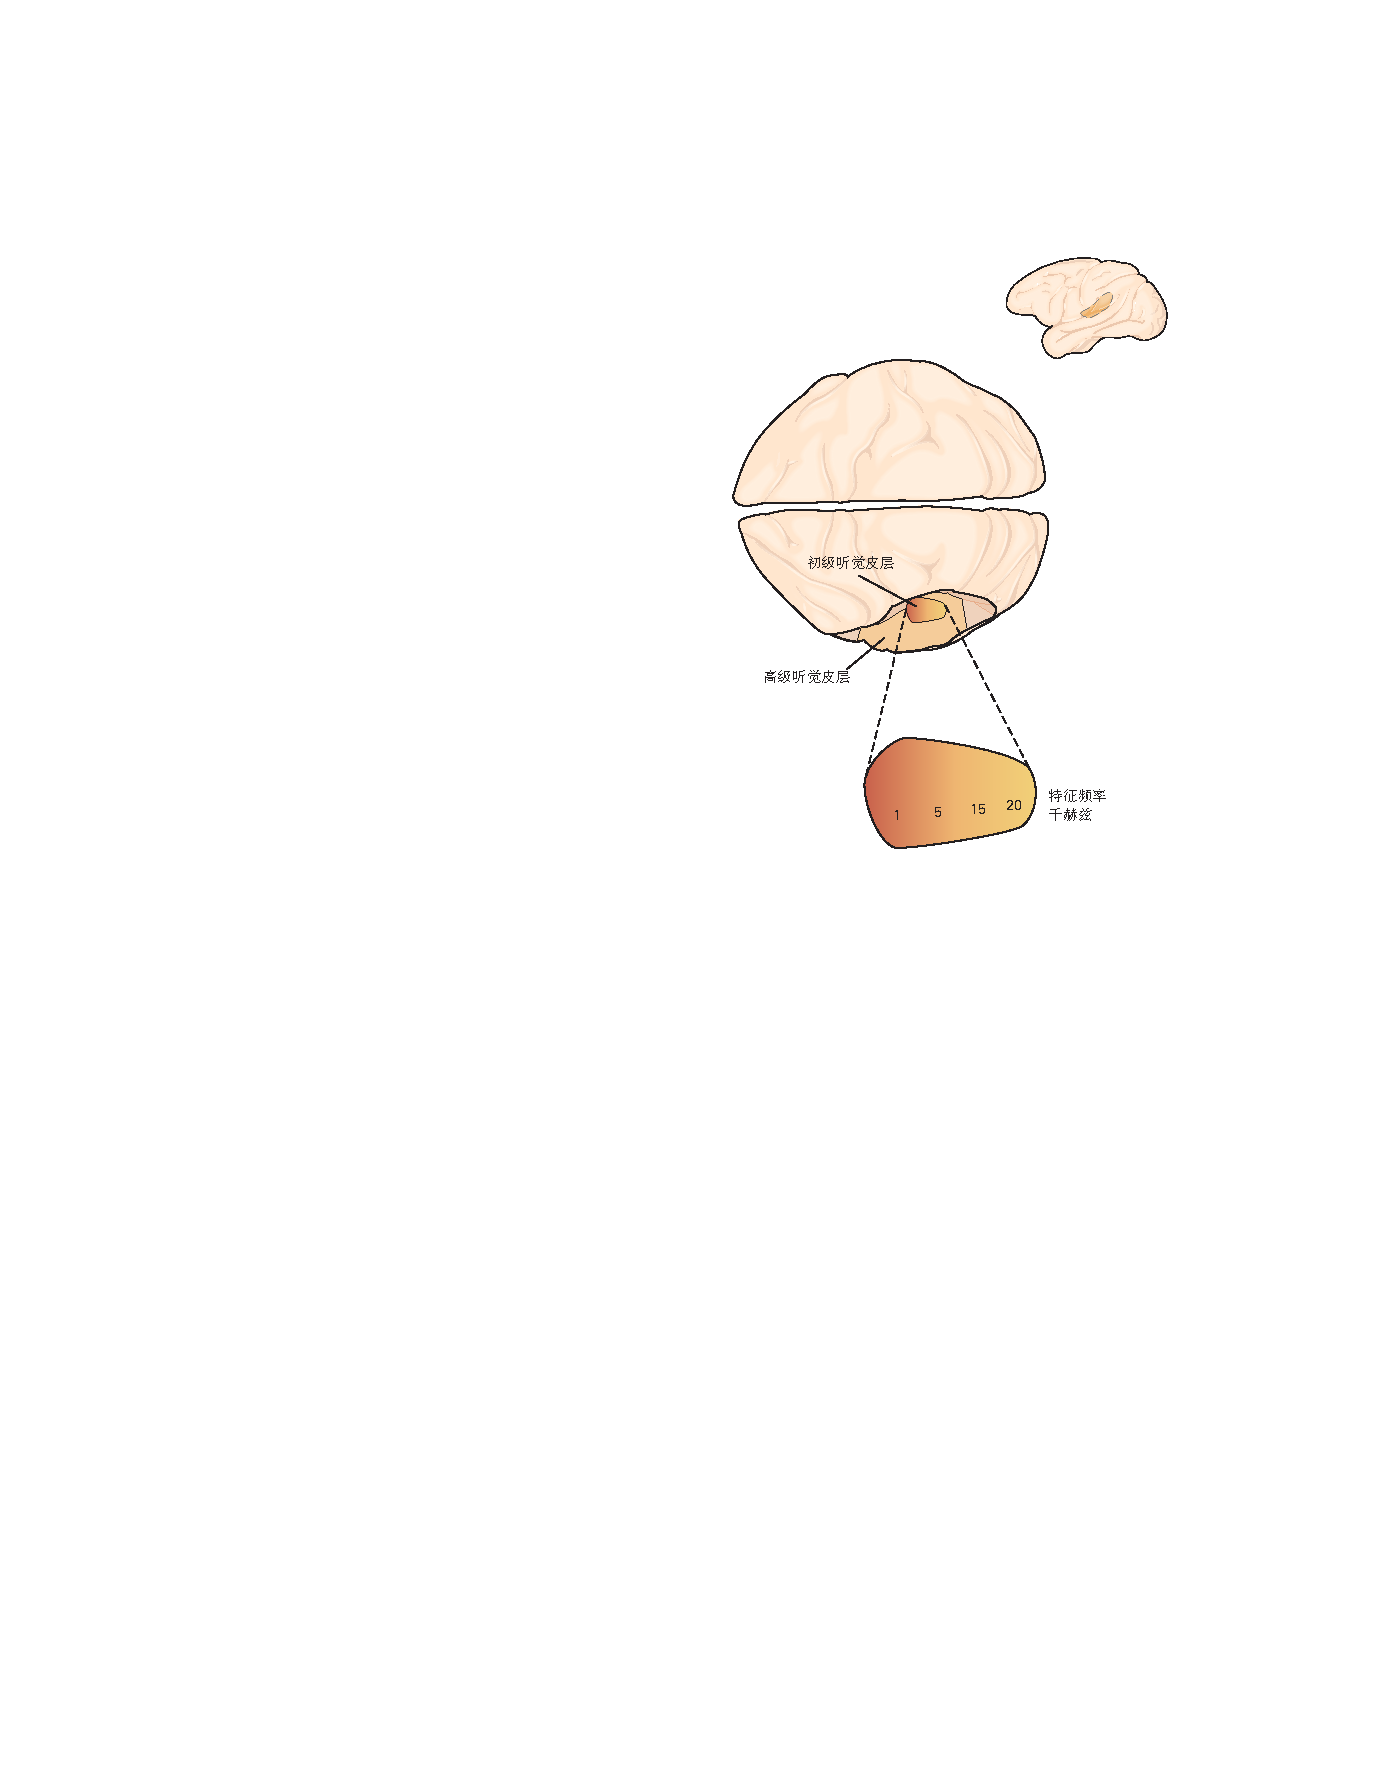
\includegraphics[width=0.5\linewidth]{chap28/fig_28_10}
	\caption{灵长类动物的听觉皮层有多个初级区和次级区。 
		初级听觉皮层的扩展图显示了它的音调组织。 主要区域被高阶区域包围(见图 28-11)。}
	\label{fig:28_10}
\end{figure}


因为耳蜗在基底膜的不同点编码离散频率,然而,外围的一维频率图分布在皮质的二维表面上,在一个方向上具有平滑的频率梯度,在另一个方向上具有等频轮廓 其他方向。 
在许多物种中,代表生物学上重要频率的听觉皮层子区域由于广泛的输入而比其他区域大,类似于初级视觉皮层中专门用于来自中央凹的输入的大区域。

除了频率之外,听觉刺激的其他特征也被映射到初级听觉皮层,尽管整体组织不如视觉清晰和精确。 
A1 中的听觉神经元被来自双耳的输入(EE 神经元)兴奋,对侧输入通常强于同侧输入,或被单侧输入 (EI) 兴奋。 
EI 神经元被对侧耳朵的刺激所抑制。

A1 中的某些神经元似乎也根据带宽进行组织,即根据它们对窄或宽频率范围的反应。 
与远离中心的神经元相比,靠近等频轮廓中心的神经元被调谐到更窄的带宽或频率。 
A1 的不同子区域形成细胞簇,在单个等频轮廓内具有窄或宽带调谐。 
在皮质内回路中,神经元主要接收来自具有相似带宽和特征频率的神经元的输入。 
这种带宽选择性的模块化组织可能允许通过不同带宽和中心频率的神经元滤波器对输入信号进行冗余处理,这可能有助于分析光谱复杂的声音,例如特定物种的发声,包括语音。

A1 中表示了其他几个参数。 
这些包括神经元反应潜伏期、响度、响度调制以及频率调制的速率和方向。 
尽管这些不同的映射如何相交还有待观察,但这个参数数组显然赋予了 A1 中的每个神经元和每个位置以表示声音的许多独立变量的能力,从而允许神经元选择性的多样性。

与皮层的视觉和体感区域一样,A1 中的感觉表征可以响应输入通路的改变而改变。 
外周听力损失后,A1 中的音调映射可以改变,这样以前对听力损失范围内的声音有反应的神经元将开始对相邻频率做出反应。 
Michael Merzenich 和其他人的工作表明,成年动物的行为训练也可以导致听觉皮层的大规模重组,因此与行为最相关的频率——那些与注意力或强化特别相关的频率——变得过多。

幼小动物的听觉区域特别具有可塑性。 
在啮齿类动物中,A1 的频率组织在早期粗略的频率图的发育过程中逐渐出现。 
在暴露于特定频率的重复音调脉冲的声学环境中饲养动物会导致专门用于该频率的皮层区域持续扩张,并伴随着音调图的普遍恶化和扩大。 \\
这一结果不仅表明 A1 的发展依赖于经验,而且还提出了早期暴露于异常声音环境可能导致高级感官处理长期中断的可能性。 
更好地了解这种情况是如何发生的,以及它是否也适用于人类胎儿和婴儿,可以深入了解中枢听觉处理受损的疾病的起源和治疗,例如多种形式的阅读障碍。 
此外,通过吸引注意力或奖励来诱导成年人听觉皮层的可塑性的能力为即使在成年期的大脑修复也带来了新的希望。

哺乳动物的主要听觉区被多个不同的区域包围,其中一些是音调区域。 
相邻的 tonotopic 域具有镜像 tonotopy:tonotopy 的方向在域之间的边界处反转。 
在猴子中,多达 7 到 10 个次级(带)区域围绕着三到四个初级或类似初级(核心)区域(见图 28-11)。 
次级区域接收来自听觉皮层核心区域的输入,在某些情况下,还接收来自丘脑核的输入。 
电生理学和影像学研究证实,人类的 A1 位于颞叶外侧裂内侧的 Heschl 回。 
此外,最近的 fMRI 研究表明,在人类中,就像在猴子中一样,纯音主要激活核心区域,而带区域的神经元更喜欢复杂的声音,例如窄带噪声突发。


\subsection{从下丘而来的第二声音定位通路涉及凝视控制的大脑皮层}
听觉皮层中的许多神经元具有广泛的空间调谐,但在对清醒动物进行研究时也发现了具有窄空间调谐的神经元。 
在猴子中,听觉皮层神经元被调谐到额叶空间和后部空间(在视觉覆盖范围之外),以及水平面上方和下方的空间。 
然而,与听觉中脑相比,尚无证据表明在任何对声音位置敏感的皮层区域中都有空间组织的声音图。

皮质中的声音定位通路起源于下丘的中央核,并通过听丘脑以及初级和次级皮质区域上升,最终到达参与注视控制的额叶眼区。 
眼睛或头部的运动可以通过刺激前额眼区来引起,前额眼区直接连接到介导凝视变化的脑干被盖运动前核以及上丘。 
但是,当从下丘的位置敏感神经元到上丘的中脑通路直接控制头部、眼睛和耳朵的定向运动时,为什么还要有第二个声音定位通路连接到凝视控制电路呢?

行为实验阐明了这个问题。 
虽然 A1 的病变会导致严重的声音定位缺陷,但当任务只是通过推动杠杆来指示声源的一侧时,不会出现任何缺陷。 
只有当动物必须接近短暂声源的位置时,缺陷才会变得明显; 也就是说,当任务是形成源图像、记住它并朝着它移动的更复杂的任务时。

对谷仓猫头鹰的实验产生了特别有说服力的证据。 
猫头鹰在空间中定位声音的能力不受鸟类额叶眼场等价物失活的影响。 
同样,当中脑声音定位通路被上丘的药理失活所破坏时,准确转头的可能性会降低,但动物仍然有一半以上的时间会做出正确反应。 
相反,当两个结构都失活时,动物完全无法准确定位对侧的声音刺激。 
因此,皮层和皮层下声音定位通路可以并行访问注视控制中心,或许提供了一些冗余。 
此外,当只有额叶视区失活时,鸟类就失去了将目光转向已经消失且必须记住的目标的能力,就像在哺乳动物 A1 病变中看到的那样。 
因此,在哺乳动物和鸟类中,更复杂的声音定位任务都需要皮层通路。

这似乎是皮质和皮质下通路之间的一般差异。 
皮层下电路对于快速可靠地执行对生存至关重要的行为非常重要。 
皮层电路允许工作记忆、复杂的识别任务、刺激的选择和对其重要性的评估,从而导致更慢但更差异化的表现。 
这方面的例子也存在于不涉及本地化的听觉通路中。 
对简单听觉刺激的条件性恐惧反应是由从听觉丘脑到杏仁核的直接快速通路介导的; 它们仍然可以在皮质失活后被引出。 
然而,需要更复杂的听觉刺激辨别力的恐惧反应需要通过大脑皮层的通路,因此速度较慢但更具体。

\subsection{大脑皮层中的听觉回路被分离成分开的处理流}
在视觉系统中,初级视觉皮层的输出被分成独立的背侧和腹侧流,分别与物体在空间中的位置和物体识别有关。 
人们认为体感皮层中也存在类似的分工,最近的证据表明听觉皮层也遵循这一规划。

对猴子中三个最容易接近的带区的解剖学追踪研究表明,更多的嘴侧和腹侧区域主要连接到颞叶的更多的嘴侧和腹侧区域,而更多的尾侧区域投射到背侧和尾侧颞叶。 
此外,这些腰带区域及其颞叶目标都投射到额叶的大部分不同区域(图\ref{fig:28_11})。

\begin{figure}[htbp]
	\centering
	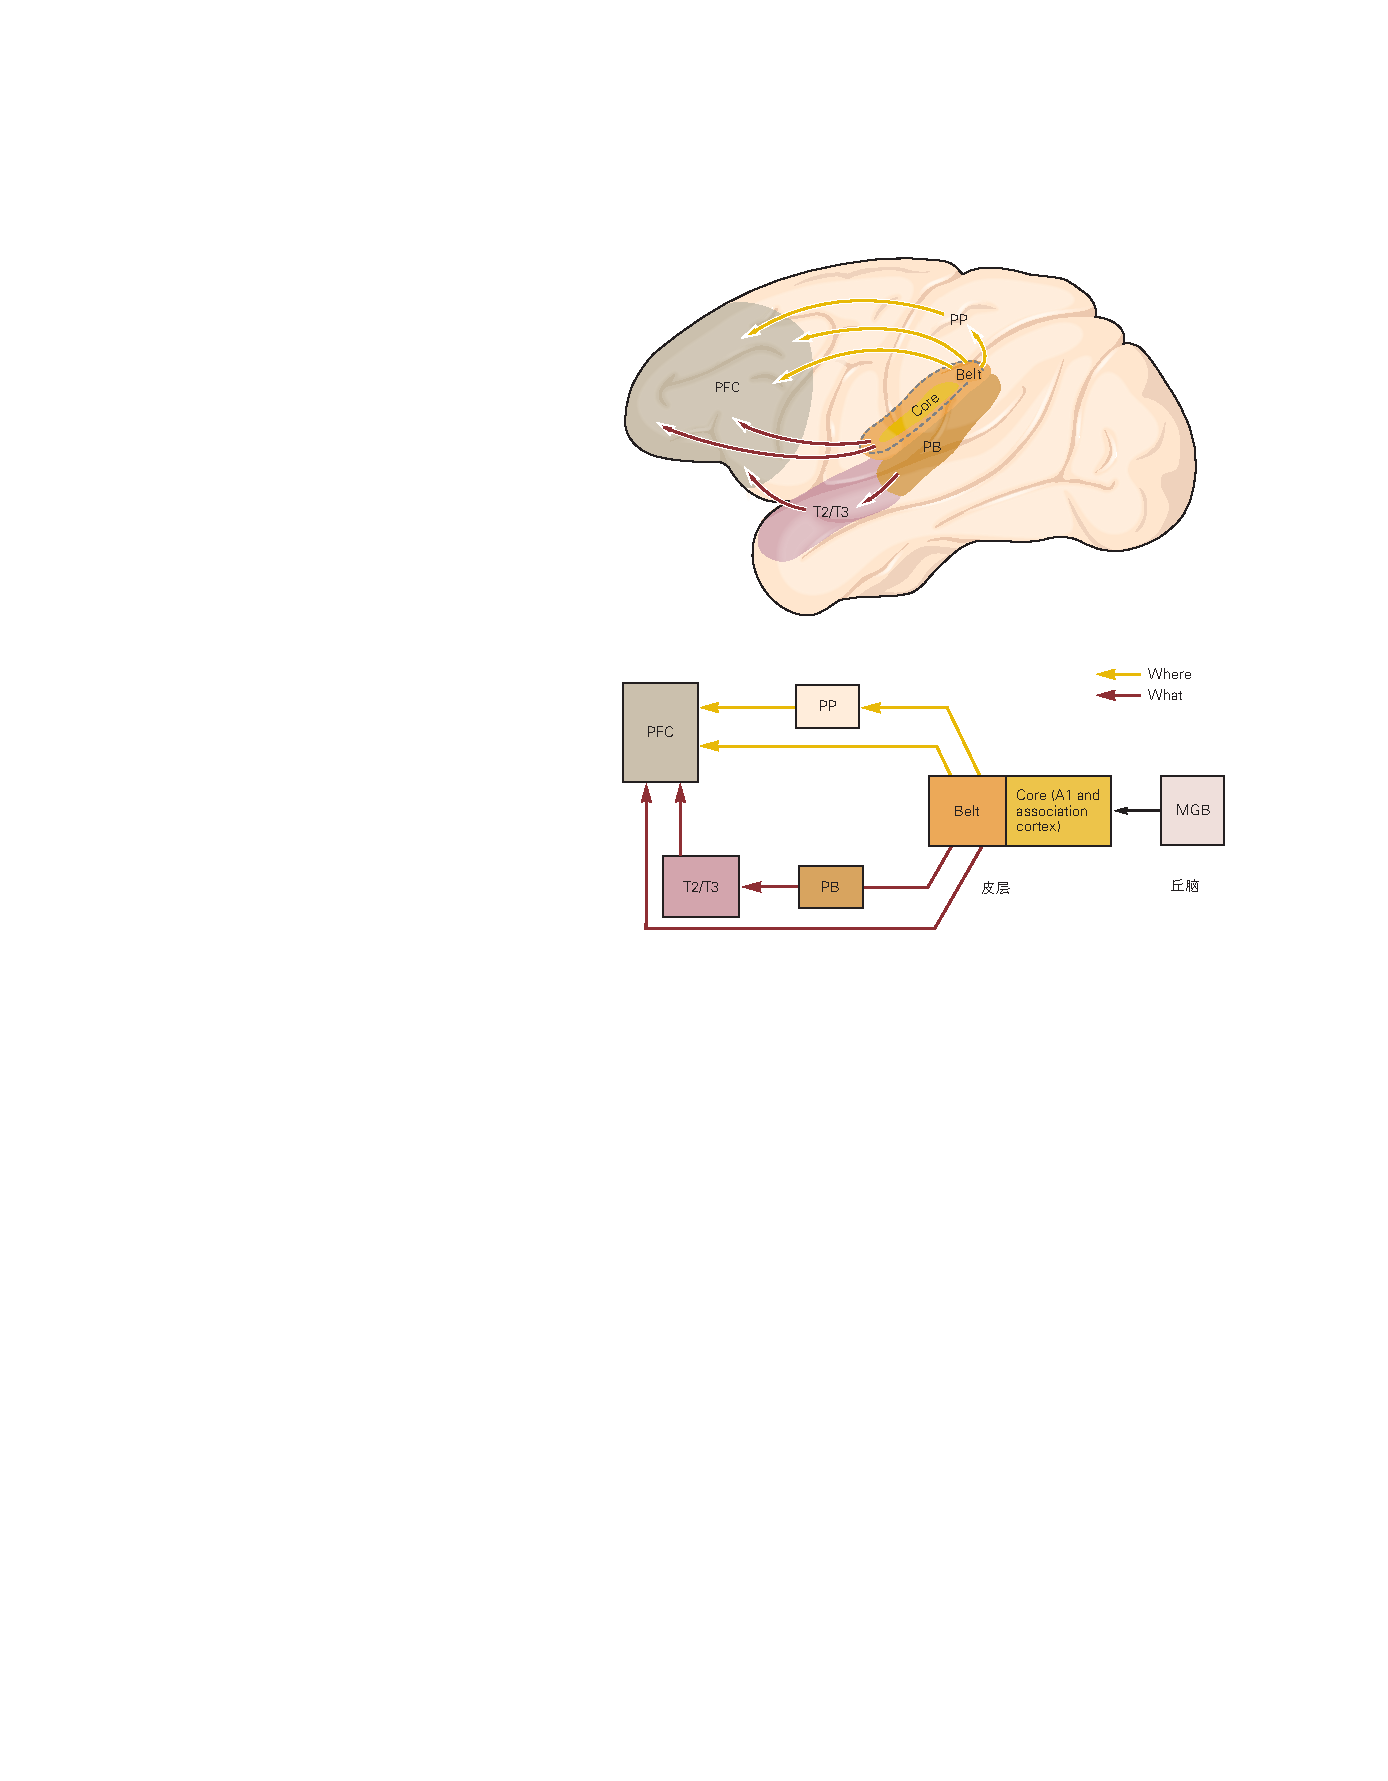
\includegraphics[width=0.5\linewidth]{chap28/fig_28_11}
	\caption{“什么”和“哪里”在灵长类动物的听觉皮层系统中流动。 
		腹侧“什么”流和背侧“哪里”流起源于初级和带状皮层的不同部分,并最终通过独立路径投射到前额叶皮层的不同区域。
		(MGB,丘脑内侧膝状体;PB,副带皮层;PFC,前额叶皮层;PP,后顶叶皮层;T2/T3,颞叶皮层区域。)
		(经许可改编自 Rauschecker 和 Tian 2000。
		版权所有 2000 美国国家科学院;改编自 Romanski 和 Averbeck 2009。)}
	\label{fig:28_11}
\end{figure}

接收前听觉投射的额叶区域通常与非空间功能有关,而那些作为后听觉区域目标的额叶区域则与空间处理有关。 
电生理学和影像学研究为此提供了支持。 
当必须定位或移动刺激时,尾部和顶叶区域更加活跃,而腹侧区域在识别相同刺激或分析其音调时更加活跃。 
因此,前-腹侧通路可以通过分析声音的频谱和时间特征来识别听觉对象,而更多的背侧-后侧通路可能专注于声源定位、声源运动检测和声源的空间分离。

尽管大脑皮层的所有感觉区域最初都将物体识别和定位分开的想法很有吸引力,但这可能过于简单化了。 
很明显,听觉皮层的内侧带区域投射到背侧和腹侧额叶皮质,具有广泛空间反应能力的神经元分布在整个尾部和前部区域。 
尽管如此,尽管系统之间的细节可能不同,但基本概念认为感觉系统将刺激解构为特征并在离散路径中分析每种类型。


\subsection{大脑皮层在皮下听区调制感觉加工}
所有哺乳动物皮层区域的一个有趣特征,也是听觉系统共有的一个特征,是从皮层回到较低区域的大量投射。 
进入感觉丘脑的皮质纤维数量几乎是从丘脑投射到皮质的轴突数量的 10 倍。 
来自听觉皮层的投射也支配下丘、橄榄耳蜗神经元、一些基底神经节结构,甚至耳蜗背核。

对这种反馈的可能功能的洞察来自蝙蝠的听觉系统。 
频率特异性皮层区域的沉默导致相应频率特异性区域中丘脑和下丘的反应减少,而皮层投射的激活增加并增强了一些神经元的反应。
因此,听觉皮层可以主动调整和改善皮层下结构中的听觉信号处理。 
各种证据表明,皮层反馈也发生在其他哺乳动物身上。 
这挑战了将上行感觉通路视为纯粹前馈回路的观点,并表明我们应该将丘脑和皮质视为相互关联且高度互连的回路,其中皮质对感知进行某种自上而下的控制。


\section{大脑皮层形成复杂的声音表示}


\subsection{听觉皮层使用时间编码和速率编码来表征时变声音}
听觉系统的一个重要功能是在多个时间尺度上表示随时间变化的声音,从几毫秒到几十、几百毫秒甚至更长。 
在听觉神经中,激活模式在很大程度上反映了声音的时间结构,与声音同步激活到锁相的极限。 
由于体细胞和树突的突触整合,随着信息向听觉皮层上升,这种基于时间的神经表征的精度逐渐降低。


周期性声音的锁相上限沿着上行听觉通路逐渐降低,从听觉神经中的大约 3,000 Hz 到丘脑内侧膝状体中的小于大约 300 Hz 和 A1 中的小于 100 Hz。 
A1 中的锁相上限与皮质的初级视觉和体感区域中的锁相上限相似。 
在听觉皮层中,单独的时间放电模式不足以代表人类和动物感知到的整个时变声音范围。


皮层神经元使用另一种方法来表示随时间变化的声音,这些声音的变化速度比 A1 中锁相的上限更快。 
当动物听到一系列周期性的咔哒声时,在 A1 中观察到两种类型的神经反应。 
一组神经元显示锁相周期性放电,以响应点击间隔较长的点击序列或缓慢变化的声音,但不会响应点击间隔较短或快速变化的声音的点击序列(图\ref{fig:28_12}A)。 
第二组神经元不会以较长的点击间隔响应点击序列,而是随着点击间隔变短而越来越快地发射(图\ref{fig:28_12}B)。 
这两个 A1 神经元群,分别称为同步和异步,具有互补的响应特性。 
同步群体的神经元通过同步神经放电(时间代码)明确表示缓慢发生的声音事件,而非同步群体的神经元通过平均放电率(速率代码)的变化隐式表示快速变化的声音事件。

\begin{figure}[htbp]
	\centering
	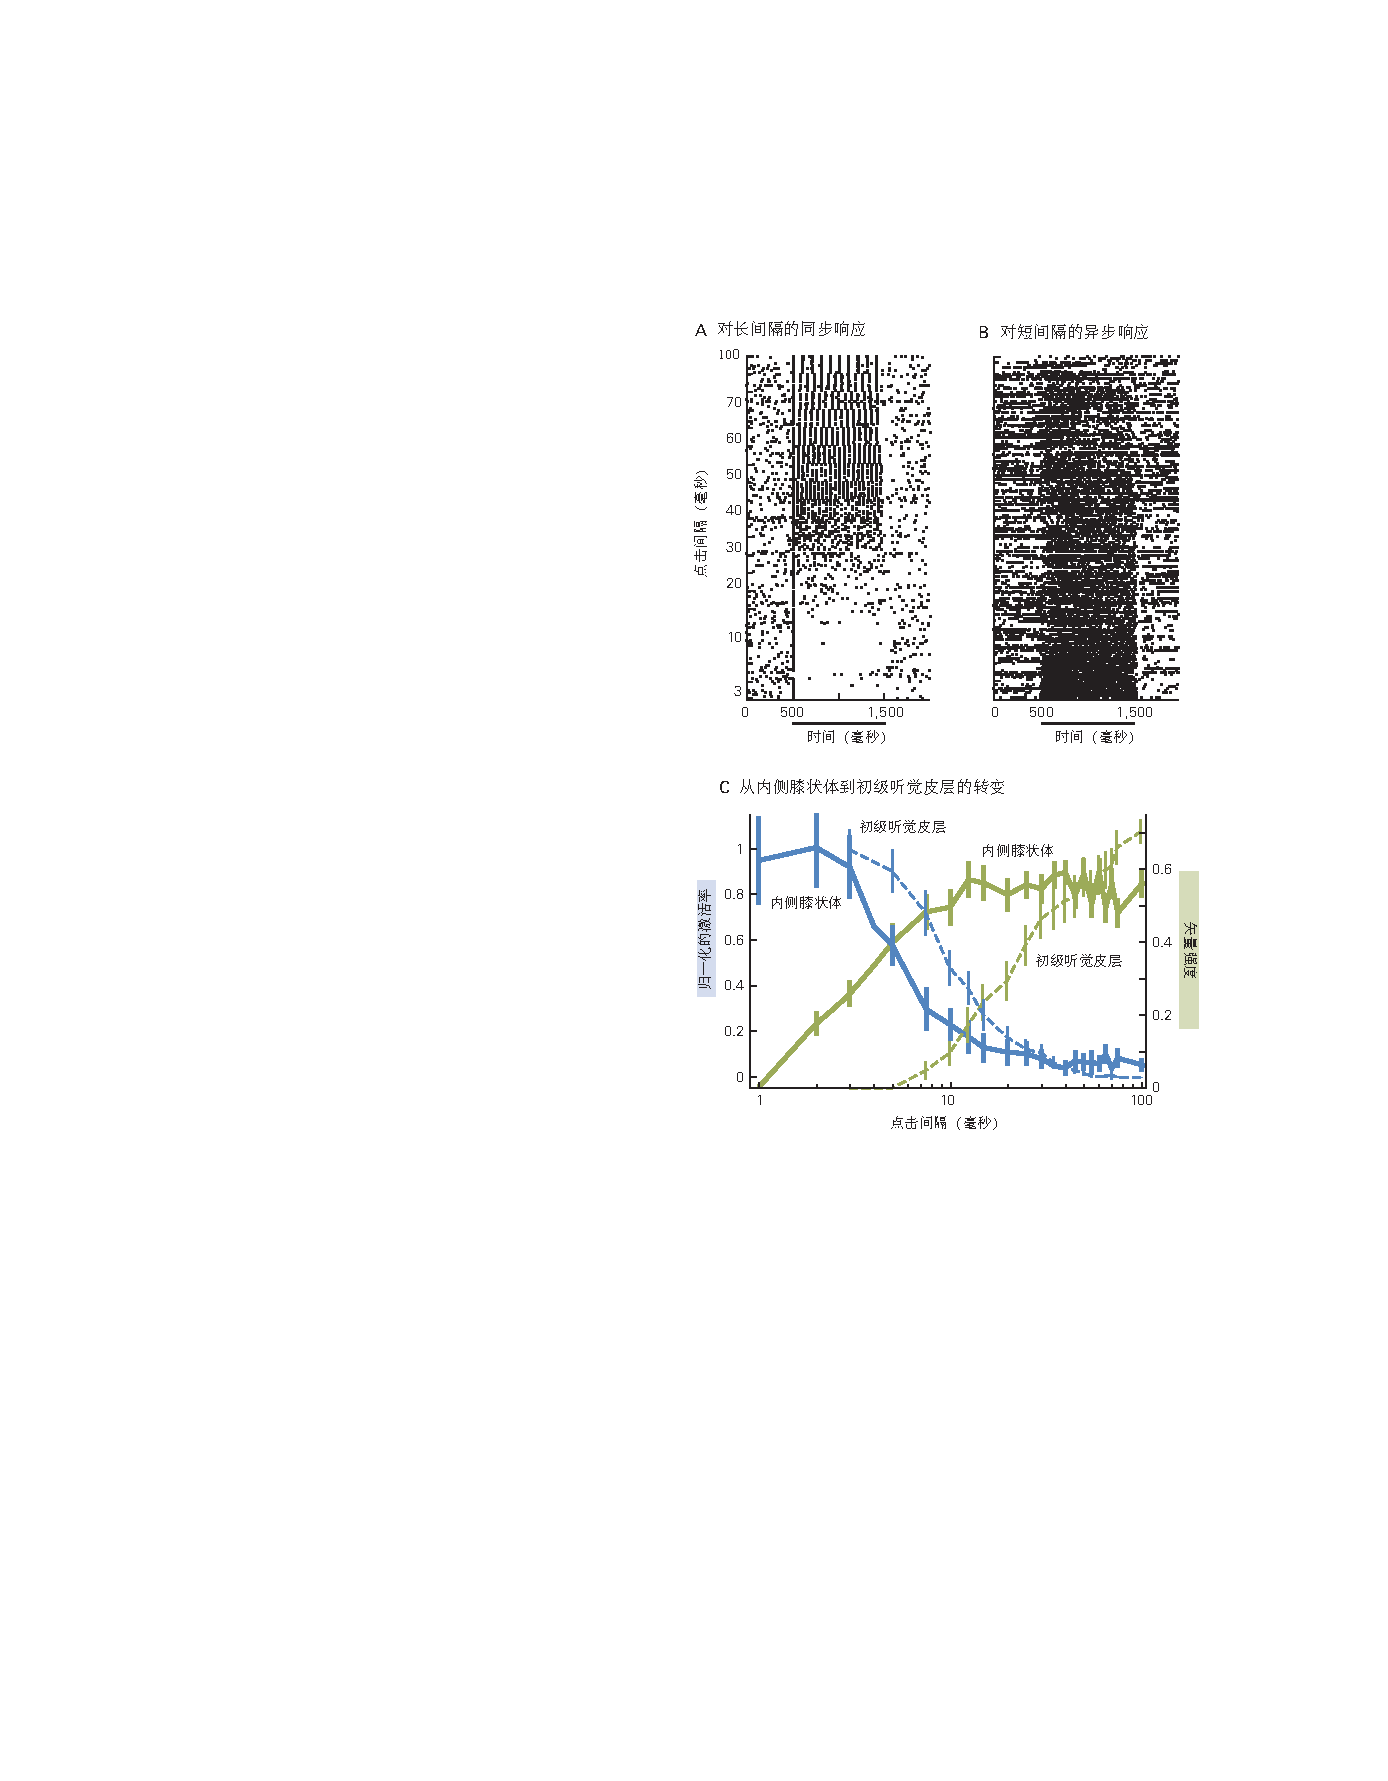
\includegraphics[width=0.5\linewidth]{chap28/fig_28_12}
	\caption{时变声音的时间编码和速率编码。
	A. 神经元对从清醒狨猴 A1 记录的周期性点击序列的刺激同步响应。 x 轴下方的水平条表示刺激的持续时间。 
	(经许可改编自 Lu、Liang 和 Wang 2001。版权所有 © 2001 Springer Nature。)
	B. 清醒狨猴 A1 记录的神经元对周期性点击序列的非同步响应。 
	(经许可改编自 Lu、Liang 和 Wang 2001。
	版权所有 © 2001 Springer Nature。) 
	C. 初级听觉皮层 (A1) 和丘脑内侧膝状体 (MGB) 之间的时间响应特性比较。 
	刺激同步响应由矢量强度量化,矢量强度是锁相强度的量度。 
	非同步响应由归一化发射率(数据曲线标识为 A1 率和 MGB 率)量化。 
	误差线表示均值的标准差。 (经许可改编自 Bartlett 和 Wang 2007。)}
	\label{fig:28_12}
\end{figure}

\subsection{灵长类有专门的皮层神经元编码音调和泛音}
% 频率高,则音"高"
音调感知对于感知语音和音乐以及在复杂的声学环境中识别听觉对象至关重要。 
音调是一种感知,可以让和谐结构的周期性声音在音阶上被感知和排序。 
音调在汉语等有声调语言中携带重要的语言信息,在欧洲语言中携带韵律信息。 
我们使用音调来识别鸡尾酒会中嘈杂背景中的特定声音。 
聆听管弦乐队时,我们会在伴奏乐器的背景下听到独奏者的旋律。

% 机械波的音高即为基波波长,但基波的强度大小却不一定大过谐波强度大小,有时基波的强度大小甚至为零,这种情形即为基频缺失。
理解音调的一个重要现象是对“基频缺失”的感知,也称为剩余音高。 
当一起演奏基频的谐波时,即使基频缺失,音高也会被视为基频。 
例如,200 Hz 基频的谐波在 400、600、800 Hz 等处。 
一起播放 400、600 和 800 Hz 的频率将产生 200 Hz 的音高感知,即使声音中实际上不存在 200 Hz 的明显频率分量。 
当我们通过太小而无法发出低频声音的扬声器听音乐时,我们经常会遇到这种现象。

许多频率组合可以产生共同的基频或音调,使其成为特别有价值的听觉线索。 
这在音调传达行为重要信息时特别有用,例如人类语言或动物发声的情况。 
通过环境传播的声音可能会发生频谱退化,失去高频或低频。 
虽然这种频谱过滤会扭曲频谱信息,但尽管损失了一些谐波分量,但对缺失基波的感知仍然很稳健。


感知音调的能力并非人类独有。 
鸟、猫和猴子也能分辨出音调。 
猴子能够辨别频谱音调、识别旋律和概括八度音阶,每一项都需要感知音调。 
狨猴是一种声音高亢的新大陆灵长类动物,其听觉范围与人类相似,表现出与人类相似的音调感知能力。 
对于 440 赫兹以上的周期,狨猴能够以小至一个半音的精度区分谐波声音中缺失的基波。


鉴于人类和某些动物都经历过一种音调,这种音调可以概括为具有相同周期性的各种声音(包括缺少基音的谐波声音),因此可以合理地预期某些神经元会从复杂的声音中提取音调。 
十年前,王晓勤和他的同事发现狨猴听觉皮层的一个小区域包含“音调选择性神经元”。 
这些神经元被调谐到具有最佳频率的纯音,并以接近其最佳频率的基频响应谐波复合体,即使谐波位于神经元的兴奋性频率响应区域之外(图\ref{fig:28_13}A)。

\begin{figure}[htbp]
	\centering
	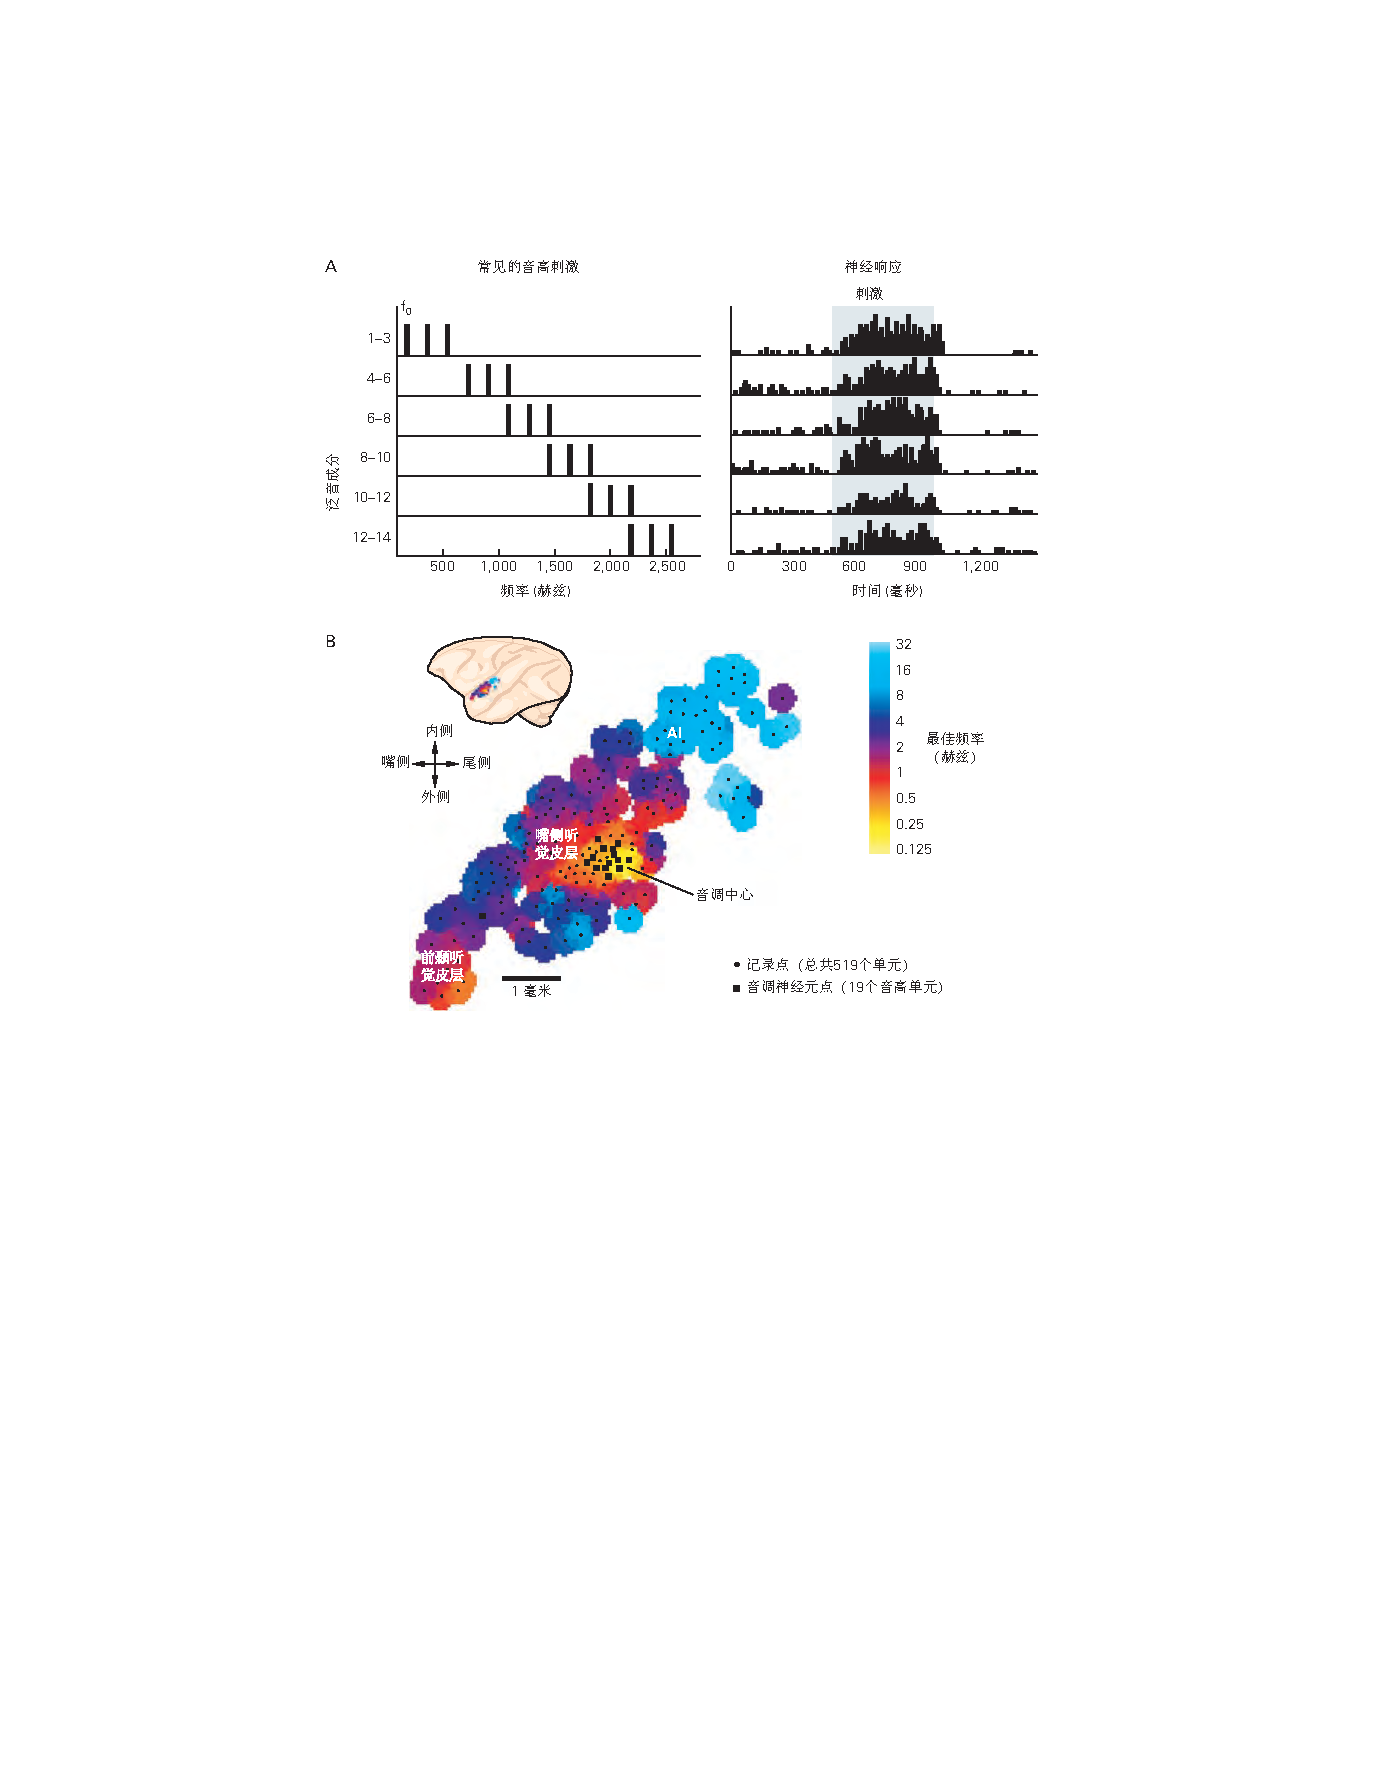
\includegraphics[width=0.5\linewidth]{chap28/fig_28_13}
	\caption{音调由灵长类动物听觉皮层中的专门神经元编码。 
		A. 从狨猴听觉皮层记录的音高选择性神经元的例子。 左图:共享相同基频 (f0) 的一系列谐波刺激的频谱。 右图:神经元对刺激的反应的刺激周时间直方图(阴影区域表示的刺激持续时间)。 
		(经许可改编自 Bendor 和 Wang 2005。版权所有 © 2005 Springer Nature。) 
		B. 狨猴听觉皮层的解剖组织和音高中心的位置。 上图:狨猴大脑的侧视图。 
		底部:左听觉皮层的 Tonotopic 图以一只狨猴为特征。 
		音高选择性神经元(黑色方块)聚集在 A1 和区域 R(延髓听觉皮层)之间的低频边界附近。 
		频率反转表示 A1/R 和 R/RT(喙颞听觉皮层)之间的边界。 
		(BF:最佳频率。)(改编自 Bendor 和 Wang 2005。版权所有 © 2005 Springer Nature。)}
	\label{fig:28_13}
\end{figure}

当音调接近神经元的首选最佳频率时,音调选择性神经元会对音高唤起声音(例如,和声、咔嗒声)做出响应。 
随着音调的行为显着性增加,音调选择性神经元会增加它们的放电率,并且更喜欢周期性的声音而不是非周期性的声音。 
重要的是要注意狨猴中的音调选择性神经元,它提取和编码嵌入谐波声音中的音调(高度非线性计算),明显不同于皮层下区域或仅“反映”音高信息的 A1 神经元 在他们的激活模式中。

狨猴中包含音调选择性神经元的区域仅限于 A1 的低频边界、延髓听觉皮层(R 区)和外侧带区(图\ref{fig:28_13}B)。 
人类成像研究已经确定了位于 A1 前外侧的 Heschl 脑回外侧端的一个限制区域,该区域提取谐波复杂声音的音高,并且对音高显着性的变化敏感。 
该区域的位置反映了狨猴的俯仰中心位置(图\ref{fig:28_13}B)。


狨猴听觉皮层的核心区域也包含一类谐波模板神经元,它们对纯音或双音组合反应微弱或根本不反应,但对多重谐波的特定组合反应强烈。 
谐波模板神经元对谐波声音的反应比非谐波声音更强,并且对特定谐波结构具有选择性。 
与位于 A1 和 R 之间低频边界外侧的小皮层区域内并且最佳频率小于 1,000 Hz 的音调选择性神经元相反,谐波模板神经元分布在 A1 和 R 中并且具有最佳频率 范围从大约 1 kHz 到大约 32 kHz,这个范围涵盖了狨猴的整个听觉范围。


而在外围,单个听觉神经纤维编码谐波声音的各个分量,而谐波模板神经元的特性揭示了用于提取谐波模式的谐波结构感受野。 
从听觉神经纤维到听觉皮层的和声神经表征的变化反映了感觉系统中神经编码的原理。 
感觉通路中的神经元将物理特征的表示(例如听觉中的声音频率或视觉中的图像亮度)转换为感知特征的表示,例如听觉中的音高或视觉中的曲率。 
这些特征导致听觉或视觉知觉的形成。 
听觉皮层中的谐波模板神经元是处理具有谐波结构的声音的关键,例如动物发声、人类语言和音乐。


\subsection{食虫蝙蝠有皮层区域专门负责行为相关的声音特征}
虽然人们普遍认为上游听觉区执行与听觉相关的越来越专业的功能,但与视觉系统相比,人们对听觉系统中串行继电器的功能知之甚少。 
在人类中,听觉最重要的方面之一是它在处理语言中的作用,但我们对神经回路如何分析语音声音知之甚少。 
人类大脑成像的新技术逐渐提供了对与语言相关的皮层区域功能专业化的见解(第 55 章)。


专门分析大脑皮层中复杂听觉信号的证据来自对食虫蝙蝠的研究。 
这些动物几乎完全通过回声定位找到猎物,发出被飞虫反射的超声波脉冲。 
蝙蝠分析回声的时间和结构以帮助定位和识别目标,而离散的听觉区域专门处理回声的不同方面。


许多蝙蝠,例如 Nobuo Suga 和他的合作者研究的大胡子蝙蝠,都会发出具有两种成分的回声定位脉冲。 
初始恒定频率 (Constant-Frequency, CF) 分量由多个谐波相关的声音组成。 
这些谐波会稳定地发出几十到几百毫秒,类似于人类的元音。 
恒定频率分量之后是频率急剧下降的声音,调频 (frequency-modulated, FM) 分量,类似于人类辅音的快速变化频率(图 28-14A)。

\begin{figure}[htbp]
	\centering
	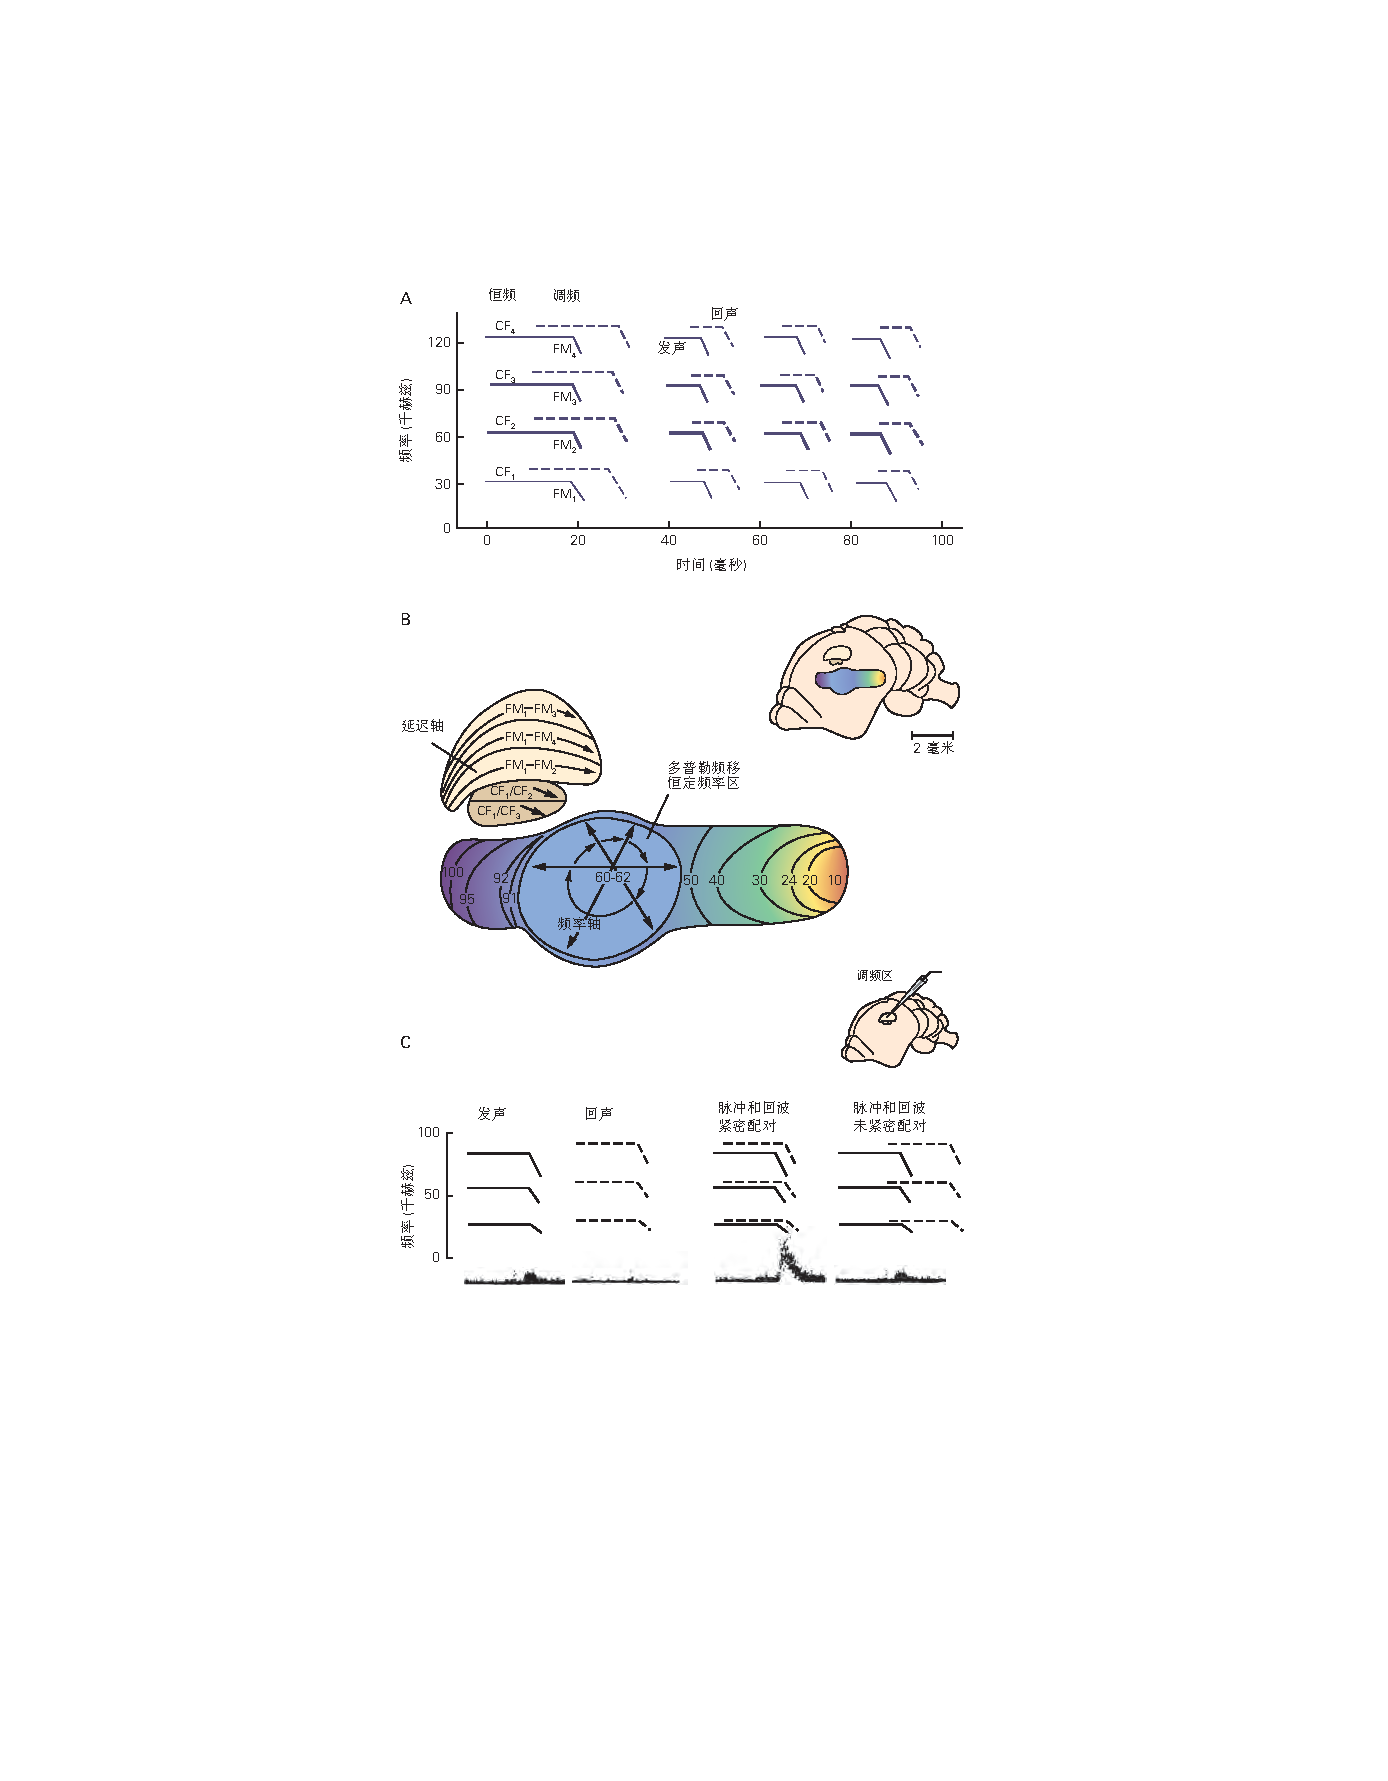
\includegraphics[width=0.5\linewidth]{chap28/fig_28_14}
	\caption{蝙蝠的听觉系统有专门的区域来定位声音。 
		A. 动物叫声声波图(实线)和由此产生的回声(虚线)说明了叫声的两个组成部分:延长的、谐波相关的恒频 (CF) 信号和较短的调频 (FM) 信号。 
		当动物接近其目标时,呼叫的持续时间会缩短。 (经许可改编自 Suga 1984。) 
		B. 大胡子蝙蝠的大脑半球视图显示了听觉皮层内的三个功能区域。 FM 区域是计算与目标的距离的地方; CF 区域是计算目标速度的地方; 多普勒频移 CF 区域专门用于识别小的颤动物体。 
		在呼叫频率 (60–62 kHz) 的二次谐波附近,多普勒频移 CF 信号的扩展皮质表示形成了声学“中央凹”。 (经许可改编自 Suga 1984。)
		C. 所示的 FM-FM 组合敏感神经元对单独的脉冲或回波没有显着响应,但对紧密配对的脉冲回波响应非常强烈。 
		然而,神经元对脉冲和回波之间的时间差也很敏感,如右侧的记录所示,神经元无法响应未紧密配对的脉冲-回波组合。 (经 Suga 等人许可改编,1983 年。)}
	\label{fig:28_14}
\end{figure}


FM 声音用于确定到目标的距离。 
蝙蝠根据相对恒定的声速测量发出的声音和返回的回声之间的间隔,该间隔对应于特定距离。 
听觉皮层 FM-FM 区域的神经元(图\ref{fig:28_14}B)优先响应由特定延迟分隔的脉冲回波对。 
此外,这些神经元对特定声音组合的反应比对单独声音的反应更好。 
这样的神经元被称为特征检测器(图 28-14C)。 
FM-FM 区域包含一系列此类检测器,首选延迟系统范围为 0.4 至 18 毫秒,对应于 7 至 280 厘米的目标范围(图 28-14B)。 
这些神经元按列组织,每个列都对刺激频率和延迟的特定组合有反应。 
通过这种方式,蝙蝠就像其下丘中的谷仓猫头鹰一样,能够表现出一种听觉特征,而这种特征不能直接由感觉感受器表现出来。


蝙蝠叫声的 CF 分量用于确定目标相对于蝙蝠的速度和目标的声学图像。 
当回声定位蝙蝠飞向昆虫时,从昆虫反射的声音在蝙蝠耳中被多普勒频移到更高频率,因为蝙蝠正朝着从目标返回的声波移动,导致这些声音相对加速 在它的耳边挥手。 
同样,一只后退的昆虫会在蝙蝠的耳朵处产生频率降低的反射。 
CF-CF 区域(图 28-14B)中的神经元被急剧调谐到接近发射频率或其谐波的频率组合。 
每个神经元对特定基频的脉冲与对应于脉冲的一次或二次谐波的回波的组合反应最好,多普勒频移到特定程度。 
与 FM-FM 区域一样,神经元不会单独响应脉冲或回波,而是响应两个 CF 信号的组合。

CF-CF 神经元按列排列,每个列编码特定的频率组合。 
这些列沿皮层表面规则排列,基频沿一个轴,回声谐波沿垂直轴。 
这种双频坐标系创建了一个地图,其中特定位置对应于特定的多普勒频移,因此对应于特定的目标速度,范围从 –2 m/s 到 9 m/s。


返回回波的 CF 分量也用于声学图像的详细频率分析,可能在其识别中很重要。 
胡须蝙蝠的多普勒频移恒频区 (DSCF) 是初级听觉皮层对 60 kHz 至 62 kHz 频率表示的显着扩展,与来自蝙蝠的主要 CF 成分的一组返回回声很好地对应 呼叫(图 28-14B)。 
在 DSCF 区域内,单个神经元被极其敏锐地调谐到频率,因此很容易检测到飞蛾翅膀颤动所产生的微小频率变化。


当蝙蝠执行辨别任务时,这些专门的皮层区域中的一些暂时失活,这显着地支持了它们在行为中的功能专业化的重要性。 
DSCF 的沉默有选择地削弱精细频率歧视,同时保持时间感知完好无损。 
相反,FM-FM 区域的失活会削弱蝙蝠检测两个回声到达时间的微小差异的能力,同时保持频率感知不变。


对与蝙蝠相关的刺激的了解极大地促进了对这种听觉系统的研究。 
这些皮层区域在功能上或解剖学上是否类似于猫、猴子和人类的特定区域还有待观察。 
无论如何,选择合适的刺激物在研究这些其他物种时可能与在蝙蝠研究中一样重要。


\subsection{听觉皮层涉及处理说话时的声音反馈}
声音交流包括说话和听觉,通常同时发生。 
当我们说话时,我们的声音不仅会传递给预期的听众,还会传回我们自己的耳朵。 
在发声过程中,这种对我们听觉系统的反馈不仅通过空气进行,还通过骨骼进行,并且由于嘴和耳朵的接近而可能很响亮。


听觉系统必须区分听觉感知是自我产生的还是外部产生的。 
为了在说话过程中监测来自声学环境的外部声音,必须屏蔽自身产生的声音。 
同时,听觉系统还必须监测我们自己的声音,以检测发声中的错误。 
通过声音反馈准确表达自己的声音对于保持理想的发声和学习新语言至关重要。 
在人类和动物中,声音反馈的扰动会导致声音产生的改变,而声音反馈的中断或阻塞会导致声音学习的退化。

听觉皮层参与处理声音反馈的证据来自人类和动物研究。 
说话时人类受试者的听觉皮层对自己声音的反应小于对相同声音回放的反应。 
这种减少可以在脑电图 (ECoG) 记录(图 28-15A)或各种成像方法(例如,fMRI、PET、脑磁图 [MEG])中观察到。

\begin{figure}[htbp]
	\centering
	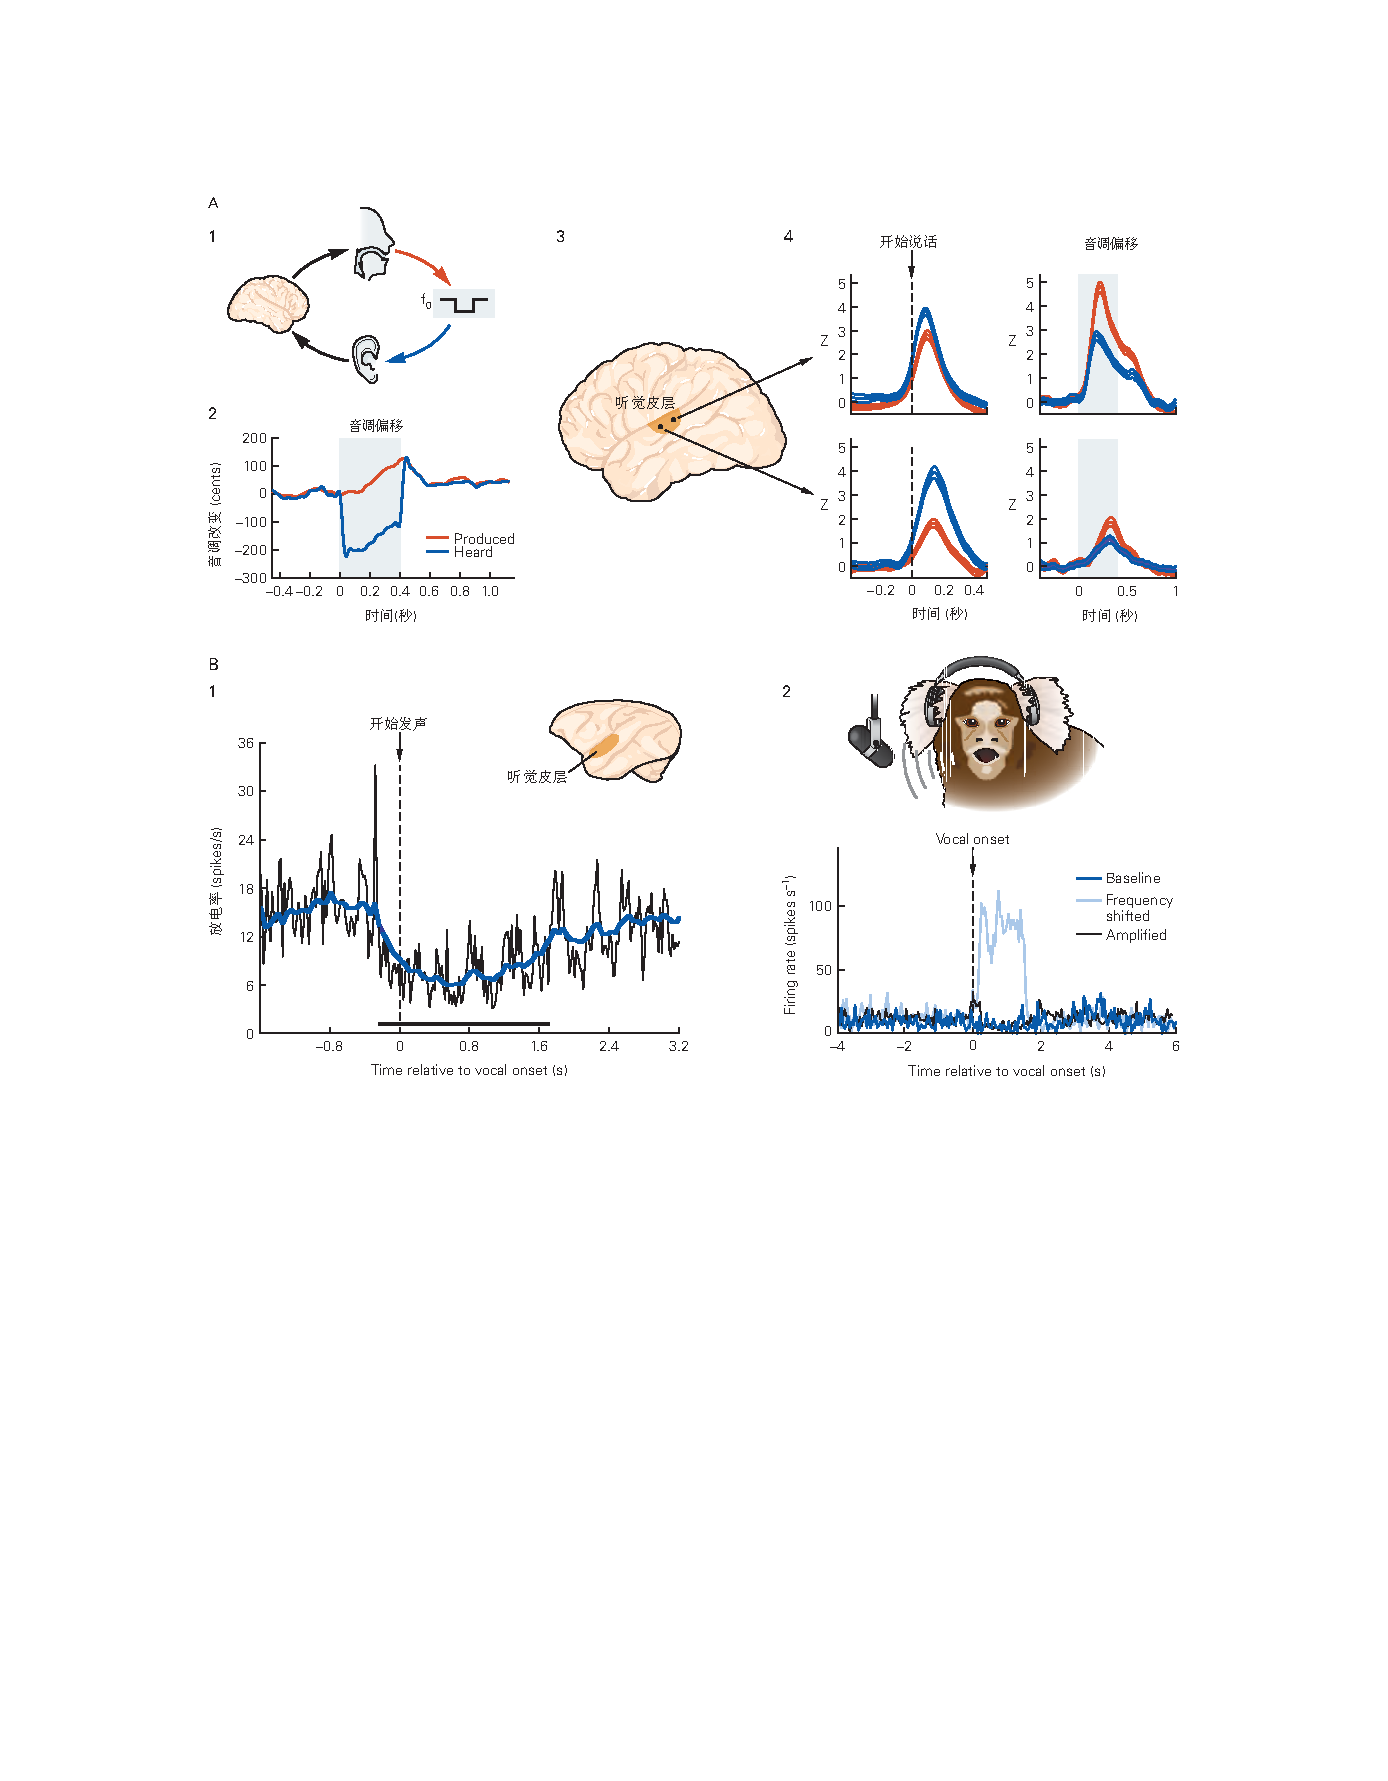
\includegraphics[width=0.5\linewidth]{chap28/fig_28_15}
	\caption{听觉皮层的声音反馈处理。 
	A. 发声引起的抑制和对人类大脑皮层音调扰动的敏感性的例子。 
	1. 受试者的发声(红色箭头)通过数字信号处理器,该处理器改变音调并将失真的听觉反馈(蓝色箭头)传送到受试者的耳机。 
	2. 示例试验的音调轨迹显示了麦克风记录的音调(产生)和传送到耳机的音调(听到)。 
	阴影区域表示信号处理器将音高移动 −200 音分(1 音分 = 1/1200 倍频程)时的时间间隔。 
	3. 从颞上回表面听觉皮层的两个位置记录的电极位置。 
	4. Z 变量表示皮层活动在 50 至 150 Hz(高 γ)范围内的功率,这已被证明与神经元尖峰活动密切相关。 
	它是从每个电极在说话(红色)和听力(蓝色)条件下记录的信号中提取的。 
	图左栏中的垂直线表示发声开始,图右栏中的阴影区域表示扰动的开始和偏移。 
	受试者的听觉皮层对其自己发声的反应通常小于受试者被动聆听相同发声回放时的反应(左栏)。 
	听觉皮层在主动发声(说话)期间对扰动的反应得到增强(右栏)。 (
	经许可改编自 Houde 和 Chang,2015 年。)
	B. 1. 发声诱导的狨猴听觉皮层神经活动抑制。 
	所有发声抑制反应的人口平均发射率与发声(“Phee”呼叫)一致。 
	蓝线是移动平均值(100 毫秒窗口),表明抑制在发声之前开始(用箭头表示)。 
	粗条表示抑制持续显着的时期(P <0.05)。 (经许可改编自 Eliades 和 Wang 2003。) 
	2. 受到发声诱导抑制的神经元对声音反馈扰动很敏感。 
	上图:通过定制的耳机将带或不带反馈改变的自制发声传送到狨猴。 
	底部:这个听觉皮层神经元在正常发声(深蓝色)期间被抑制,但当发声的听觉反馈在频域(浅蓝色)中移动时,其放电率显着增加。 
	单独放大听觉反馈不会产生放电率变化(黑色)。 (经许可改编自 Eliades 和 Wang 2008;Crapse 和 Sommer 2008。)}
	\label{fig:28_15}
\end{figure}


来自发声猴听觉皮层的单神经元记录表明,自发发声导致皮质对猴子自身发声的反应、发声期间听到的外部声音以及自发活动的抑制(图 28-15B)。 因为在许多情况下,放电率被抑制到低于自发活动,抑制很可能是由抑制引起的。 被自发发声抑制的神经元表现出频率和强度调谐,这是听觉皮层神经元的典型特征,并对发声的回放做出反应。

发声诱导的抑制在发声开始前几百毫秒开始(图 28-15B),表明这些神经元接收来自发声电路的调制信号。 在人类中,声音的产生是由额叶的皮层区域进行的,从布罗卡区到前运动和运动皮层。 在人类和猴子中,已经描述了从运动前皮层到颞上回听觉区的轴突,并且据推测,它们介导了发声诱导的抑制。 当人类或猴子只是聆听播放给它们的声音时,这种调节连接并不活跃。

为什么我们说话时会抑制听觉皮层? 一个简单的答案是,这种抑制有助于降低我们自己声音的掩蔽效果,这种声音可能非常响亮。 一个更有趣的答案是,这种抑制是由听觉皮层中的声音反馈监控网络引起的。 在人类中,如果通过耳机实验性地改变声音反馈,例如,当声音的音高发生变化时,听觉皮层的抑制就会减少或没有(图 28-15A)。 在狨猴中,当动物听到自己的频移发声时,被自发发声抑制的神经元可能变得不那么抑制甚至兴奋(图 28-15C)。 这种对反馈扰动的敏感性表明,表现出发声诱导抑制的神经元是负责监测声音反馈信号的网络的一部分。 人类和猴子听觉皮层中声音反馈相关神经活动的存在表明听觉皮层结合了内部调制和声音反馈反应,而不仅仅是对通过耳朵传来的感觉信号做出反应。

并非听觉皮层中的所有神经元都会因说话或发声而受到抑制。 狨猴 A1 中较小比例 (~30\%) 的神经元在自发发声期间增加了它们的反应,这与其听觉反应特征一致。 与发声诱导的抑制相反,发声相关的兴奋在发声开始后开始,并且可能是通过上行听觉通路反馈的结果。 与发声相关的兴奋可能有助于在说话或发声期间保持听觉皮层对外部声学环境的敏感性。

已经在几种哺乳动物皮层下结构(包括脑干和下丘)中观察到发声诱导的听觉反应抑制。 这种抑制在声音产生前几毫秒开始或与声音产生同步。 相比之下,皮层抑制在发声前几百毫秒就开始了。 说话或发声期间听觉反应的皮层下抑制可能是由皮层指令启动的。


\section{要点}
1. 撞击两只耳朵的声音携带着大脑用来计算声音出现位置及其含义的信息。 声音的特征在于一个或多个频率的能量大小。 为了确定声音在水平面的何处出现,许多哺乳动物计算小于大约 3,000 赫兹的声音到达两只耳朵的时间差异。 为了确定声音在垂直方向上出现的位置以及它们是从前面还是后面发出,哺乳动物使用头部、肩部和外耳对大于大约 6,000 Hz 的声音进行频谱过滤。 

2. 听觉神经纤维将声音信息从耳蜗传送到大脑,每条神经纤维都被急剧调谐到一个狭窄的频率范围,并共同代表动物的整个听觉范围。 听觉神经纤维终止于腹侧和背侧耳蜗核,将声学信息分配给四个主要的主要细胞群,形成通过脑干的平行上升通路。 听觉神经输入的地形组织赋予同侧耳蜗核一个音调组织,该组织在整个听觉通路(包括听觉皮层)中得到保留。 

3. 沿着上升路径的处理站处的听觉神经元的一个显着特征是它们逐渐增加的刺激选择性。 

4. 腹侧耳蜗核提取声音的三个特征:(a) 通过腹侧耳蜗核、上橄榄核和外侧丘系腹侧核的章鱼细胞的单耳通路检测听觉神经纤维的同步放电,这有助于 检测声音的开始和间隙。 (b) 星状细胞检测并锐化光谱峰谷的编码,并将光谱信息传递给背侧耳蜗核、外侧丘系腹核、外侧丘系腹侧核、下丘和丘脑中的橄榄耳蜗神经元。 频谱信息用于理解声音的含义和定位其来源。 (c) 浓密细胞锐化并传递有关声音精细结构的信息,这些信息用于通过内侧和外侧上橄榄核的双耳通路,以对两只耳朵的声音时间和强度进行耳间比较,用于 沿方位角定位声源。 

5. 耳蜗背侧核在其主要细胞中整合声学信号和体感信息。 体感信息有助于将动物自身运动产生的光谱线索与环境产生的光谱线索区分开来,这些线索在生物学上是无趣的。 

6. 听觉脑干通路汇聚于下丘。 下丘通过丘脑的内侧膝状体向听觉皮层提供声学信息。 

7. 来自下丘的投射将关于声音位置的信息传送到上丘,上丘是控制头部和眼睛的反射性定向运动的大脑的一部分。 

8. 在听觉皮层内,听觉神经元继续变得对它们响应的刺激更具选择性。 听觉皮层的子区域代表不同的生物学重要特征,例如形成谐波复合体的音高。 听觉皮层还将快速变化的声音特征转换为基于发射率的表示,同时使用尖峰时间表示缓慢变化的声音。 

9. 大脑皮层中的听觉回路被分成不同的处理流,背侧和腹侧流分别与声音在空间中的定位和声音识别有关。 

10. 大脑皮层调节皮层下听觉区的处理。 来自听觉皮层的投射支配丘脑、下丘、橄榄耳蜗神经元、一些基底神经节结构,甚至耳蜗背核。 

11. 听觉皮层参与处理说话时的声音反馈信号。 说话会抑制听觉皮层的神经活动,这种活动在发声前几百毫秒就开始了。 这种抑制是声音反馈监测网络的结果,该网络的作用是指导声音的产生和学习。


\subsection{选读}
\subsection{参考文献}
